%
% main.tex -- Paper zum Thema Autotune
%
% (c) 2019 Hochschule Rapperswil
%
\chapter{Autotune\label{chapter:autotune}}
\lhead{Autotune}
\begin{refsection}
\chapterauthor{Cédric Renda}

\definecolor{codegreen}{rgb}{0,0.6,0}
\definecolor{codegray}{rgb}{0.5,0.5,0.5}
\definecolor{codepurple}{rgb}{0.58,0,0.82}
\definecolor{backcolour}{rgb}{0.95,0.95,0.92}

\lstdefinestyle{mystyle}{
	backgroundcolor=\color{backcolour},   
	commentstyle=\color{codegreen},
	keywordstyle=\color{magenta},
	numberstyle=\tiny\color{codegray},
	stringstyle=\color{codepurple},
	basicstyle=\footnotesize,
	breakatwhitespace=false,         
	breaklines=true,                 
	captionpos=b,                    
	keepspaces=true,                 
	numbers=left,                    
	numbersep=2pt,                  
	showspaces=false,                
	showstringspaces=false,
	showtabs=false,                  
	tabsize=2
}
\lstset{style=mystyle}
\lstdefinestyle{mystyle}{
	morekeywords={cwt,contourf,datetick}
}


\section{Einleitung}
\rhead{Einleitung}
%
% einleitung.tex
%
% (c) 2018 Prof Dr Andreas Müller
%
\chapter*{Einleitung\label{chapter:einleitung}}
\lhead{Einleitung}
\addcontentsline{toc}{chapter}{Einleitung}
Zeitabhängige Signale können verstanden werden als Funktionen $t\mapsto f(t)$
mit $t\in\mathbb R$.
Die Analysis lehrt eine Reihe von Methoden, wie man mit solchen
Funktionen arbeiten kann.
Dies ist jedoch eine mathematische Idealisierung.
In der Praxis kennt man nur das Resultat eines Abtastprozesses, wo
der Funktionswert $f(t_k)$ für diskrete Werte $t_i=t_0 + k\Delta t$
ermittelt wird.
Insbesondere gehen alle Informationen über den Verlauf einer Funktion $f(t)$
zwischen den Abtastpunkten $t_k$ verloren.
Trotzdem führt daran nichts vorbei, denn nur auf diese Art ist es möglich,
Signale in einem digitalen System zu verarbeiten.

Die Methoden der Analysis sind für folgen von Abtastwerten $x_k=f(t_k)$
fast nutzlos.
Sogar das Konzept der Frequenz ist fragwürdig, denn ein Sinus-Signal
$s(t)=\sin(2\pi t/\Delta t)$ nimmt auf allen Abtastpunkten $t_k$
den Wert $s(t_k)=\sin(2\pi t_0/\Delta t+2\pi k)=\sin(2\pi t_0/\Delta t)$
den gleichen Wert an.
Allgemeiner: ein Signal mit der gleichen Frequenz wie die Abtastfrequenz
ist nicht von einem konstanten Signal unterscheidbar.
Die Signalverarbeitung verlang daher nach einem Satz von Werkzeugen, die
einerseits mit dieser Schwierigkeit fertig werden, aber andererseits auch
in der Lage sind gut verstandene technische Prozesse wie das Ausfiltern
bestimmter Frequenzbereiche adäquat zu beschreiben.

Das übliche und für den Ingenieur naheliegende Werkzeug ist die 
Fourier-Theorie, die ursprünglich als analytisches Hilfsmittel zur Lösung
von Differentialgleichungen entwickelt wurde.
Sie machte erstmals möglich, ein Signal über die darin vertretenen
Frequenzen zu charakterisieren und zu manipulieren.
Mit der Entwickung der schnellen Fourier-Transformation
(Fast Fourier Transform, FFT) wurde ihr praktischer Einsatz in digitalen
Problemlösungen möglich.
Sie bringt die neue Idee in die Diskussion, ein Signal als Überlagerung
von Beispielfunktionen zu betrachten, die besonderes einfach zu
verstehen sind.
Konkret sind dies die Funktionen $\sin kt$ und $\cos kt$ mit
$k\in\mathbb N$ bei der Analyse periodischer Signale,
oder allgemeiner die Funktion $t\mapsto e^{ikt}$ mit $k\in\mathbb Z$
bei beliebigen Signalen.
Die daraus entwickelte Theorie ist zwar sehr reichhaltig und auch erfolgreich,
aber doch in einem Punkt unbefriedigend.
Die Fourier-Transformation liefert zu einem Signal detaillierte Information
über die darin enthaltenen Frequenzen, dafür gehen aber Informationen
darüber verloren, wann interessante Ereignisse eingetroffen sind.
Die Information ist nicht ganz verloren, da sie immer noch in den Phasen
der Koeffizienten stecken, aber sie sind für alle praktischen Zwecke 
nicht mehr nutzbar, da nur über eine Rücktransformation wieder erschliessbar.

Es stellt sich daher die Frage, ob es Möglichkeiten der Analyse von Signalen
gibt, die nicht so radikal sind.
Enthält ein Signal hohe Frequenzen, dann ändert sich das Signal rasch.
Ein kurzes Ereignis passt auf diese Beschreibung, aber eine wesentliche
Eigenschaft ist damit nicht beschrieben, nämlich wann es statt gefunden hat.
Kann man Informationen über die in einem Signal vertretenen Frequenzen gewinnen,
ohne auf Information darüber verzichten zu müssen, wann diese Ereignisse
eingetreten sind?

Für eine umfassende Antwort müssen mehrere Teilfragen untersucht werden.
\begin{enumerate}
\item
Welche Arten von Vergleichssignalen soll man verwenden, um solche kurzlebigen
Ereignisse zu beschreiben?
Die trigonometrischen Funktionen sind zweifellos naheliegend und ihre
analytischen Eigenchaften einladend, doch ihre unendliche Ausdehnung entlang
der Zeitachse torpedieren von vornherein die Möglichkeit der zeitlichen
Lokalisierung von interessanten Ereignissen.
Gibt es Funktionen, die ähnliche oszillatorische Form haben
aber trotzdem über hilfreiche analytische Eigenschaften haben?
\item
Wie vergleicht man ein gegebenes Signal mit einem Vergleichssignal?
In der Fourier-Theorie lernt man einen ausgedehnten Satz von Integralformeln
zur Berechnung der Fourier-Koeffizien\-ten.
Wie müssen diese verallgemeinert werden?
\item
Wie rekonstruiert man das Signal aus dem Resultat der Analyse?
In der Fourier-Theorie lernt man Summenformeln für die Fourierreihen
und Integralformeln für ausgedehnte Signale, doch wie ist das für 
die neuen Vergleichsfunktionen umzusetzen?
\item
Die Praxis arbeitet mit diskreten Signalen. 
Wie lässt sich die Analyse diskretisieren?
Unter welchen Voraussetzungen ist die Rekonstruktion des Signals
aus der diskreten Analyse möglich?
\item
Das Verfahren ist nur dann praktisch einsetzbar, wenn sowohl die Analyse als
auch die Synthese mit effizienten numerischen Algorithmen möglich sind.
Diese Algorithmen müssen ausserdem stabil sein, d.~h.~kleine Störungen in
den Input-Daten oder Rundungsfehler während der Durchführung des Verfahrens
dürfen sich nicht zu unbrauchbaren Resultaten aufschaukeln.
\item
Welche Vergleichssignale sind für welchen Anwendungszweck geeignet?
\end{enumerate}
Die nachkommenden Kapitel versuchen, Antworten auf diese Fragen zu
geben.

In Kapitel~\ref{chapter:geometrie} wird gezeigt, wie der Vergleich
von Funktionen gleichbedeutend ist mit dem Skalarprodukt von Vektoren.
Daraus entwickelt sich dann die Theorie der Hilberträume, der
unendlichdimensionalen komplexen Vektorräume mit Skalarprodukt.
% Diese bilden den geometrischen Rahmen, in dem man die ganze 

Die bekannte Fourier-Theorie wird im Kapitel~\ref{chapter:fourier} in
den neuen Rahmen des Hilbertraumes eingeordnet.
Es demonstriert, wie die Hilbertraumtheorie die Vielfalt der vielen
verschiedenen Varianten der Fouriertheorie vereinheitlicht.

Das Haar-Wavelet ist das älteste bekannte Wavelet.
Es ist einfach und übersichtlich und kann als Beispiel für die
Phänomene dienen, die bei komplizierteren Wavelets nicht so leicht
zu verstehen sind.
Es wird in Kapitel~\ref{chapter:haar-wavelet} im Detail besprochen.

Die stetige Wavelet-Transformation analysiert ein Signal auf höchst
redundante Art.
Die Hilbert\-raum\-theorie wird in diesem Kapitel~\ref{chapter:cwt} hier
erstmals allgemeiner angewendet.
Wir lernen die Be\-ding\-ungen kennen, die nötig sind, damit ein Signal
aus seiner Wavelet-Transformation rekonstruierbar ist.
Wir geben sogar eine Formel für die Rekonstruktion an.

Bei der Diskretisierung geht Information verloren.
Das in Kapitel~\ref{chapter:shannon} diskutierte Abtast-Theorem
von Shannon gibt an, unter welchen Voraussetzungen das Signal trotz
des Informationsverlustes rekonstruierbar bleibt.

Die diskrete Wavelet-Transformation überträgt die stetige
Wavelet-Transformation auf abgetastete Signale.
Der Begriff der Multiskalen-Analyse wird in Kapitel~\ref{chapter:msa}
dazu verwendet, die angemessene Diskretisierung im ``Frequenzraum''
zu finden.

Aus der Multiskalen-Analyse lassen sich auch die schnellen Algorithmen
ableiten, welche Wavelets überhaupt erst praktisch nützlich machen.
Diese Algorithmen werden in Kapitel~\ref{chapter:algo} hergeleitet.

Selbst mit einer Multiskalen-Analyse brauchen die Algorithmen noch nicht
perfekt zu sein.
Schon bei der Fourier-Transformation war das Problem, dass zur Berechnung
der Fourier-Trans\-for\-ma\-tion alle Input-Daten notwendig sind.
Dies bedeutet, dass das Transformationsresultat erst verfügbar ist,
wenn das ganze Signal abgetastet ist.
Damit sind Verarbeitungen in Echtzeit von vornherein ausgeschlossen.
Ein Ausweg besteht darin, dass die Transformationsoperationen sich auf
einer nur sehr kleinen Anzahl Samples ausführen lassen.
Genau dies wird erreicht, wenn die verwendeten Wavelets einen kompakten Träger
haben.
Solche Wavelets wurden von Ingrid Daubechies in den neunzehnachtizger
Jahren konstruiert und waren massgebend für den schnellen Siegeszug 
der Wavelet-Transformation in den Anwendungen.

Natürlich sind die Daubechies-Wavelets nicht die einzigen praktisch
nützlichen Wavelets.
Die verbleibenden Kapitel zeigen eine Reihe von alternativen Wavelets,
zum Beispiel in Kapitel~\ref{chapter:spline} die Spline-Wavelets.
Das Haar-Wavelet ist sowohl das einfachste Daubechies-Wavelet als auch
das primäre Spline-Wavelet.











\section{Autotune mit Fourier-Transformation}
\rhead{Autotune mit Fourier-Transformation}

Die üblichste Methode um eine Frequenzanalyse über ein längeres Signal anzuwenden ist die  Kurzzeit-Fourier-Transformation oder auch short-time fourier transform, kurz STFT. Bei dieser Methode wird ein Signal, beschrieben durch $x(t)$, in kleine Zeitabschnitte zerhackt und bei jedem dieser Signalstücke eine Fourier-Transformation angwendet. Dabei wird üblicherweise die Fourier-Transformation in Anwendungen mit dem schnellen Fourier-Transformations Algorithmus berechnet.\\

Wird nun ein Element der zerhackten Funktion $x(t)$ betrachtet, kann der Start- und Endwert beliebig sein. Diese Sprünge haben bekanntlich Folgen, die im Frequenzbereich ersichtlich werden. Eine Verschmierung über die Frequenzen, auch Unschärfe genannt, ist die Folge. \\

Um dies zu verdeutlichen, wird in der Abbildung \ref{fig:Spectral} ein unendlich langes Signal $x(t)=sin(t)$(in Grau dargestellt) untersucht. 
\begin{figure}[!ht]
	\centering
	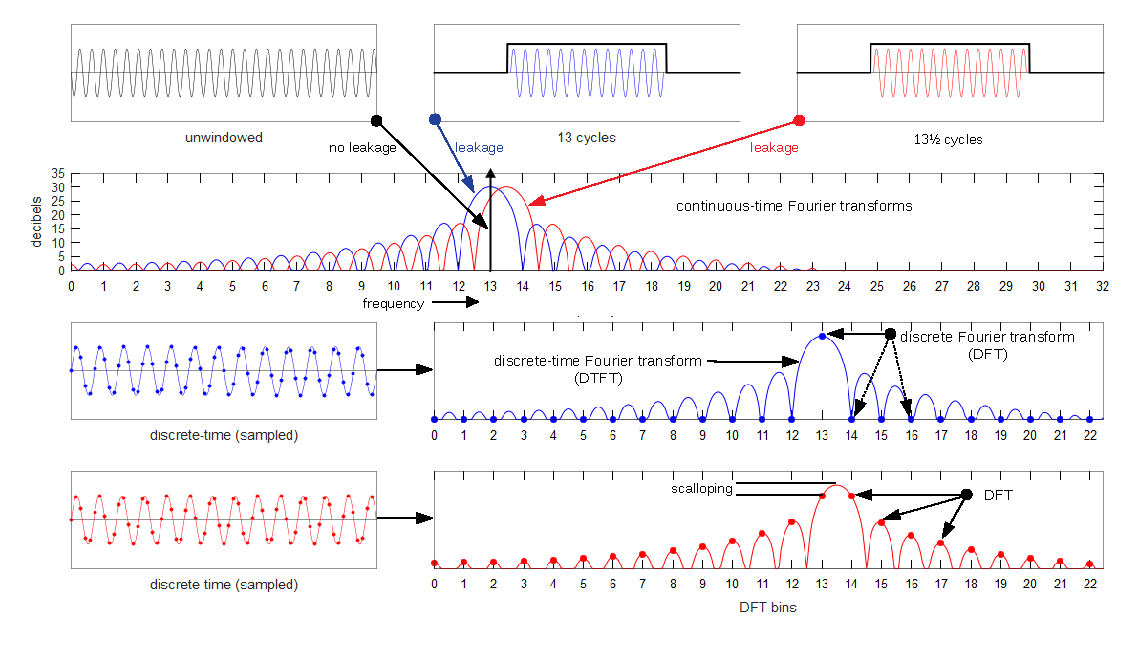
\includegraphics[scale=0.8]{papers/autotune/sections/fft/images/windows/Spectral.pdf}
	\caption{Darstellung der Fensterung und dessen mögliche Frequenzverschmierung/Unschärfe}\cite{wikipedia:Window}
	\label{fig:Spectral}
\end{figure}%

Zuerst werden die Signale zeitkontinuierlich berachtet. Im ersten Beispiel in \ref{fig:Spectral} wird das unendliche, kontinuierliche Signal $x(t)$ schwarz im Frequenzbereich abgebildet. Als Resultat erhält man nur eine Frequenz. Diese ist durch einen schwarzen Pfeil dargestellt.\\

Beim zweiten Beispiel in \ref{fig:Spectral} (in Blau) wird das Signal $x(t)$ mit der Fensterfunktion $w_{1}(t)$ multipliziert.\\
Wobei gilt: 
\begin{equation}
	w_{1}(t)= \left\{\begin{array}{lll}{t<\alpha,} & {0} \\ {\alpha\leq t \leq\beta_{1},} & {1}\\ {t>\beta_{1},}&{0}\end{array}\right\}
\end{equation}
\begin{equation}
	\hat{f_{1}}(\omega)=\frac{1}{\sqrt{2 \pi}} \int_{-\infty}^{\infty} w_{1}(t)\cdot f(t) \cdot e^{-\mathrm{i} \omega t} \mathrm{d} t
\end{equation}

$\alpha$ und $\beta_{1}$ decken ein Zeitintervall von $13$ Perioden ab. Im Frequenzbereich ist nun in Blau ersichtlich, dass die Fourier-Transformation eine deutliche Unschärfe zur Folge hat. Diese Unschärfe ist im Kontinuierlichen Spektrum ersichtlich. Das Maxima der Fouriertransformierten korreliert jedoch mit dem einen Resultat des Originalen Signales $x(t)$\\




Im letzten Fall in \ref{fig:Spectral} wird $x(t)$ mit der Fensterfunktion $w_{2}(t)$ multipliziert.\\
Wobei gilt: 
\begin{equation}
	w_{2}(t)= \left\{\begin{array}{lll}{t<\alpha,} & {0} \\ {\alpha\leq t \leq\beta_{2},} & {1}\\ {t>\beta_{2},}&{0}\end{array}\right\}
\end{equation}
\begin{equation}
	\hat{f_{2}}(\omega)=\frac{1}{\sqrt{2 \pi}} \int_{-\infty}^{\infty} w_{2}(t)\cdot f(t) \cdot e^{-\mathrm{i} \omega t} \mathrm{d} t
\end{equation}

Wobei $\alpha$ und $\beta_{2}$ ein Zeitintervall von $13\frac{1}{2}$ Perioden abdecken. Nun sieht man nicht nur eine Unschärfe sondern auch eine fehlende Korrelation zwischen dem Maxima der Fouriertansformierten und der eigentlichen Frequenz des Signales $x(t)$.\\

Betrachtet man nun die diskrete Fouriertransformierte der beiden gefensterten Signalen kann man folgendes erkenne. Ist das Signal genau über über ein vielfaches der Periode gefenstert, kann man im diskreten Fall keine Frequenzunschärfe erkennen. Trifft die Fensterung jedoch auf eine zufällige Stelle im Signal und deckt nicht gerade eine Periode ab, zeigen die diskrete Werte ein nur schwer zu interpretierbares Ergebnis an. Man spricht von einer Unschärfe. Welche nicht die eigentliche Frequenz des Signales $x(t)$ abgebildet, sondern ein ganzes Band.\\
Möchte man nun ein reales Signal Analysieren kommt es zu einem ähndlichen verhalten. Reale Signale, die meistens nicht periodisch auftreten und mit diskreten Werten beschrieben sind, werden solche Unschärfen aufzeigen. Nun gibt es verschiedenste Methoden um eine Frequenzanalyse zu realisieren. In diesem Paper wird jedoch nur auf die STFT und die Wavelet-Transformation eingegangen. 


\subsection{Zeitkontinuierliche STFT}

Das Produkt des Signals $x(t)$ mit der Fensterfunktion $w(t) $ liefert uns also eine neue Funktion die im Bereich ausserhalb des Fensters alle Werte auf null gesetzt hat. In der Anwendung sind diese Fenster meistens ein wenig überlappend damit kein Datenverlust entsteht. \\
Die Zeitkontiunierliche STFT ist  gegeben als:
\begin{equation}
	\hat{f}(\tau, \omega)=\int_{-\infty}^{\infty} x(t)\cdot w(t-\tau)\cdot e^{-j \omega t} dt
\end{equation}
mit der Kreisfrequenz  $\omega $

\subsection{Zeitdiskrete STFT}
Bei der Zeitdiskreten STFT liegt das Signal in einzelnen Abtastwerten vor. Diese Abtastwerte werden dann durch die Fensterfunktionen in einzelne Abschnitte unterteilt. \\
Die diskrete STFT ist gegeben als:
\begin{equation}
	\hat{f}(m, \omega)=\sum_{n=-\infty}^{\infty} x_{n} \cdot w_{n-m}\cdot e^{-j \omega n}
\end{equation}


\subsection{Fensterfunktionen}
Um die Unschärfe Problematik der STFT zu verbessern gibt es eine ganze Reihe an verschiedenen Fensterfunktionen die verwendet werden können um ein besseres Resultat zu erreichen. Die Auswahl der Funktion ist dabei Anwendungsspezifisch. In der Folgenden Tabelle \ref{tab:STFTtab} findet man eine kleine Auswahl mit dem jeweiligen Spektrum 


\begin{figure}[!ht]
	\begin{minipage}{.4\columnwidth}
		\textbf{Rechteck-Fenster}\\
		$w_{n}=1$
	\end{minipage}%
	\begin{minipage}{.6\columnwidth}
		\centering
		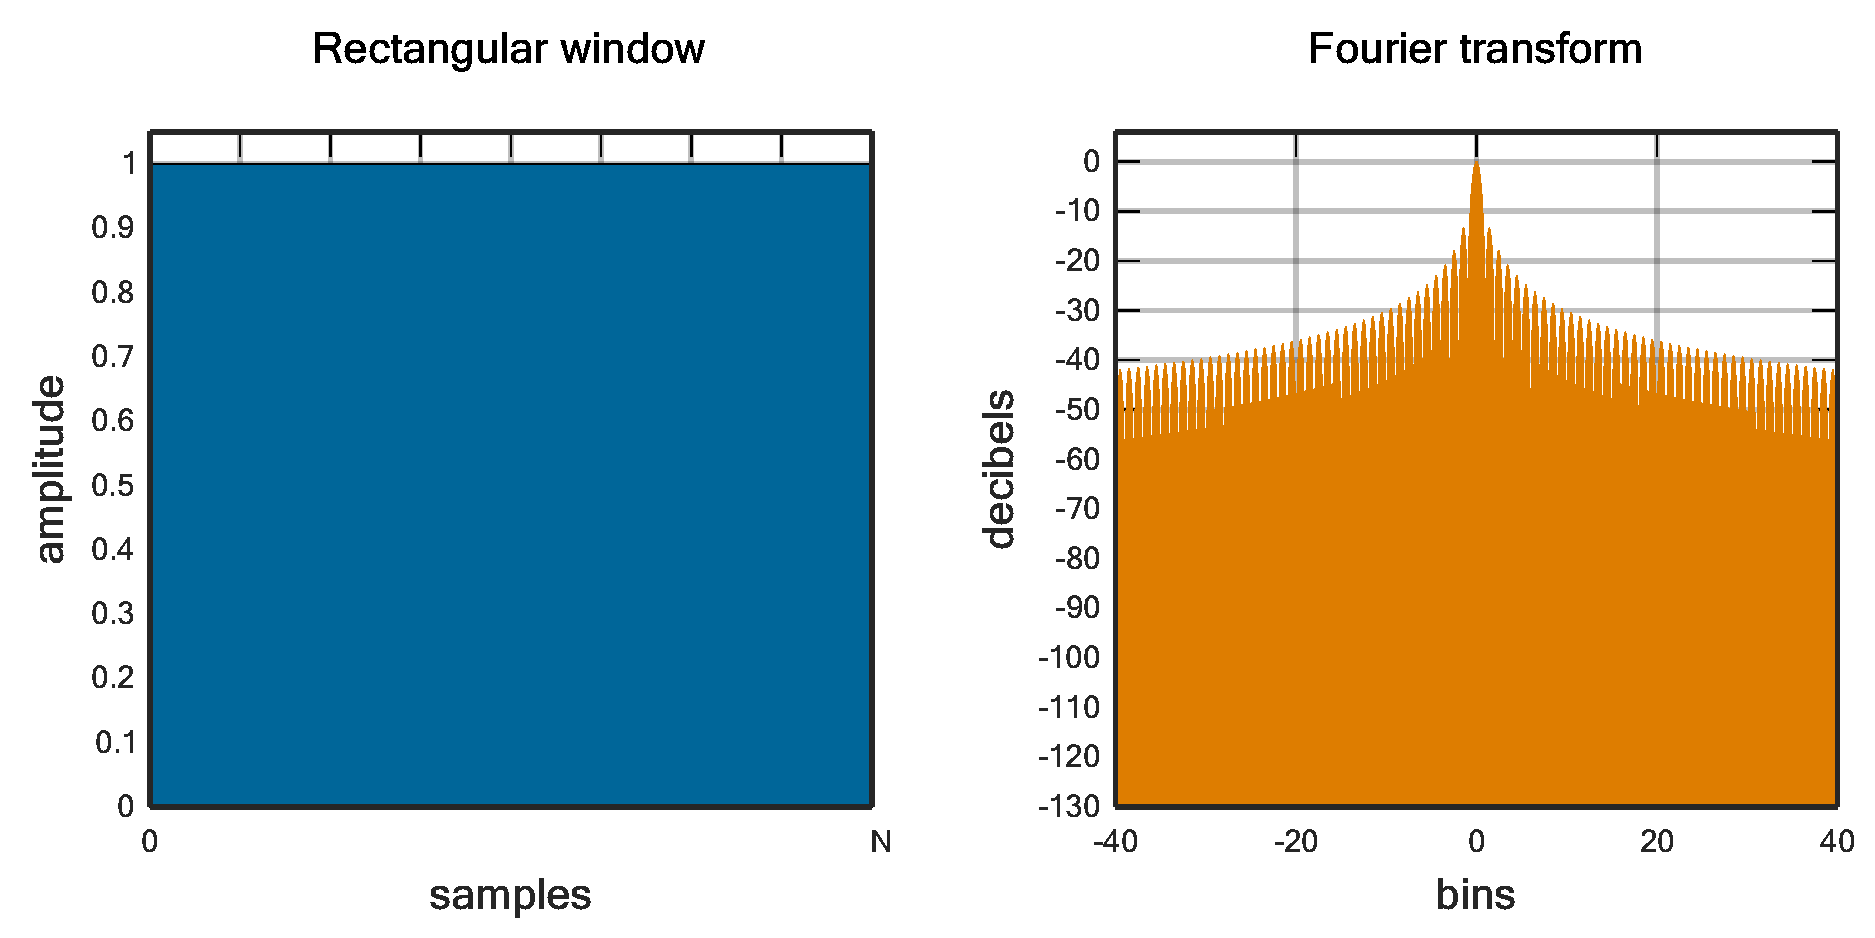
\includegraphics[width=\linewidth]{papers/autotune/sections/fft/images/windows/Rectangular.pdf}
	\end{minipage}


	\begin{minipage}{.4\columnwidth}
		\textbf{Gauss-Fenster} mit $\sigma = 0.4$\\
		$w_{n}=e^{-\frac{1}{2}\left(\frac{n-N / 2}{\sigma N / 2}\right)^{2}},$\\
		$ \quad 0 \leq n \leq N$\\
		$\sigma \leq 0.5$
	\end{minipage}%
	\begin{minipage}{.6\columnwidth}
		\centering
		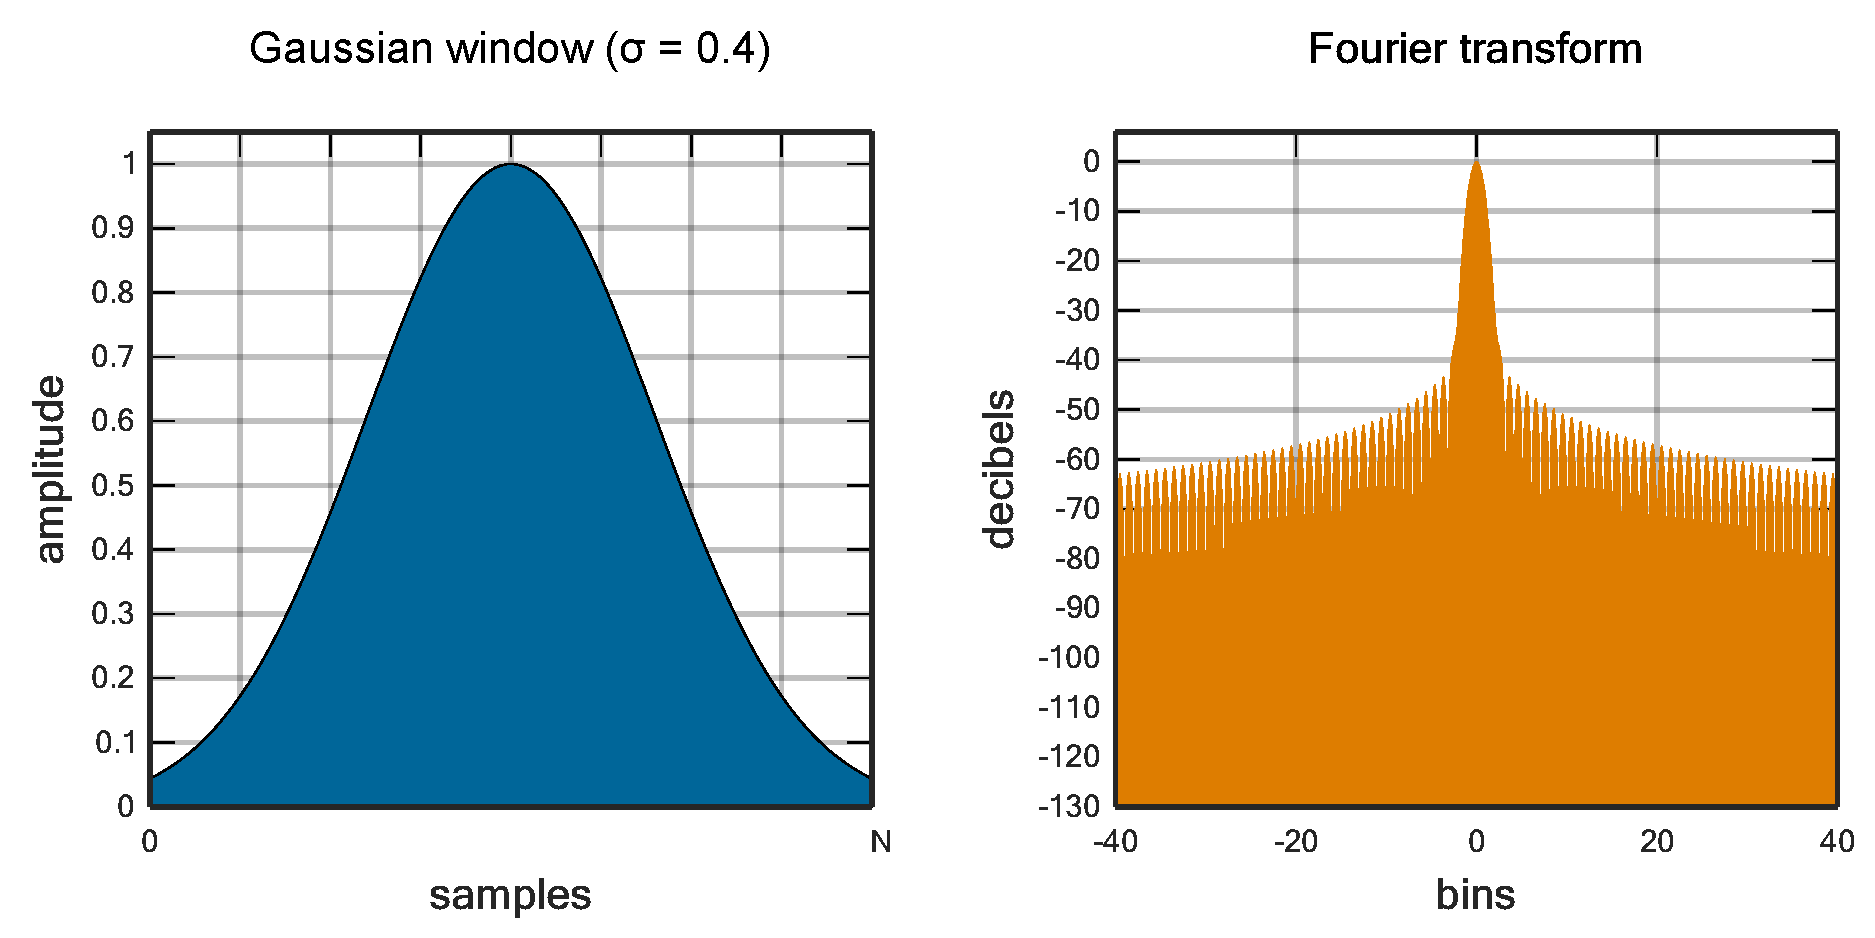
\includegraphics[width=\linewidth]{papers/autotune/sections/fft/images/windows/Gauss.pdf}
	\end{minipage}


	\begin{minipage}{.4\columnwidth}
		\textbf{Blackman-Fenster}\\
		$\begin{array}{l}{w_{n}=a_{0}-a_{1} \cos \left(\frac{2 \pi n}{N}\right)+a_{2} \cos \left(\frac{4 \pi n}{N}\right)} \\ 		{a_{0}=\frac{1-\alpha}{2} ; \quad a_{1}=\frac{1}{2} ; \quad a_{2}=\frac{\alpha}{2}}\end{array}$
	\end{minipage}%
	\begin{minipage}{.6\columnwidth}
		\centering
		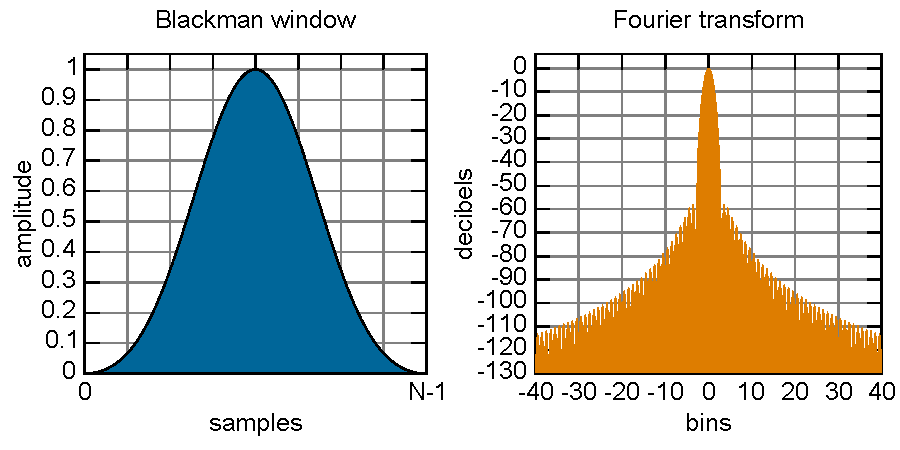
\includegraphics[width=\linewidth]{papers/autotune/sections/fft/images/windows/Blackman.pdf}
	\end{minipage}


	\begin{minipage}{.4\columnwidth}
		\textbf{Blackman-Harris-Fenster}\\
		$w_{n}=a_{0}-a_{1} \cos \left(\frac{2 \pi n}{N}\right)+a_{2} \cos \left(\frac{4 \pi n}{N}\right)-a_{3} \cos \left(\frac{6 \pi n}{N}\right)$\\
		wobei:
		$a_{0}=0.35875 ; \quad a_{1}=0.48829 ;$\\
		$ \quad a_{2}=0.14128 ; \quad a_{3}=0.01168$
	\end{minipage}%
	\begin{minipage}{.6\columnwidth}
		\centering
		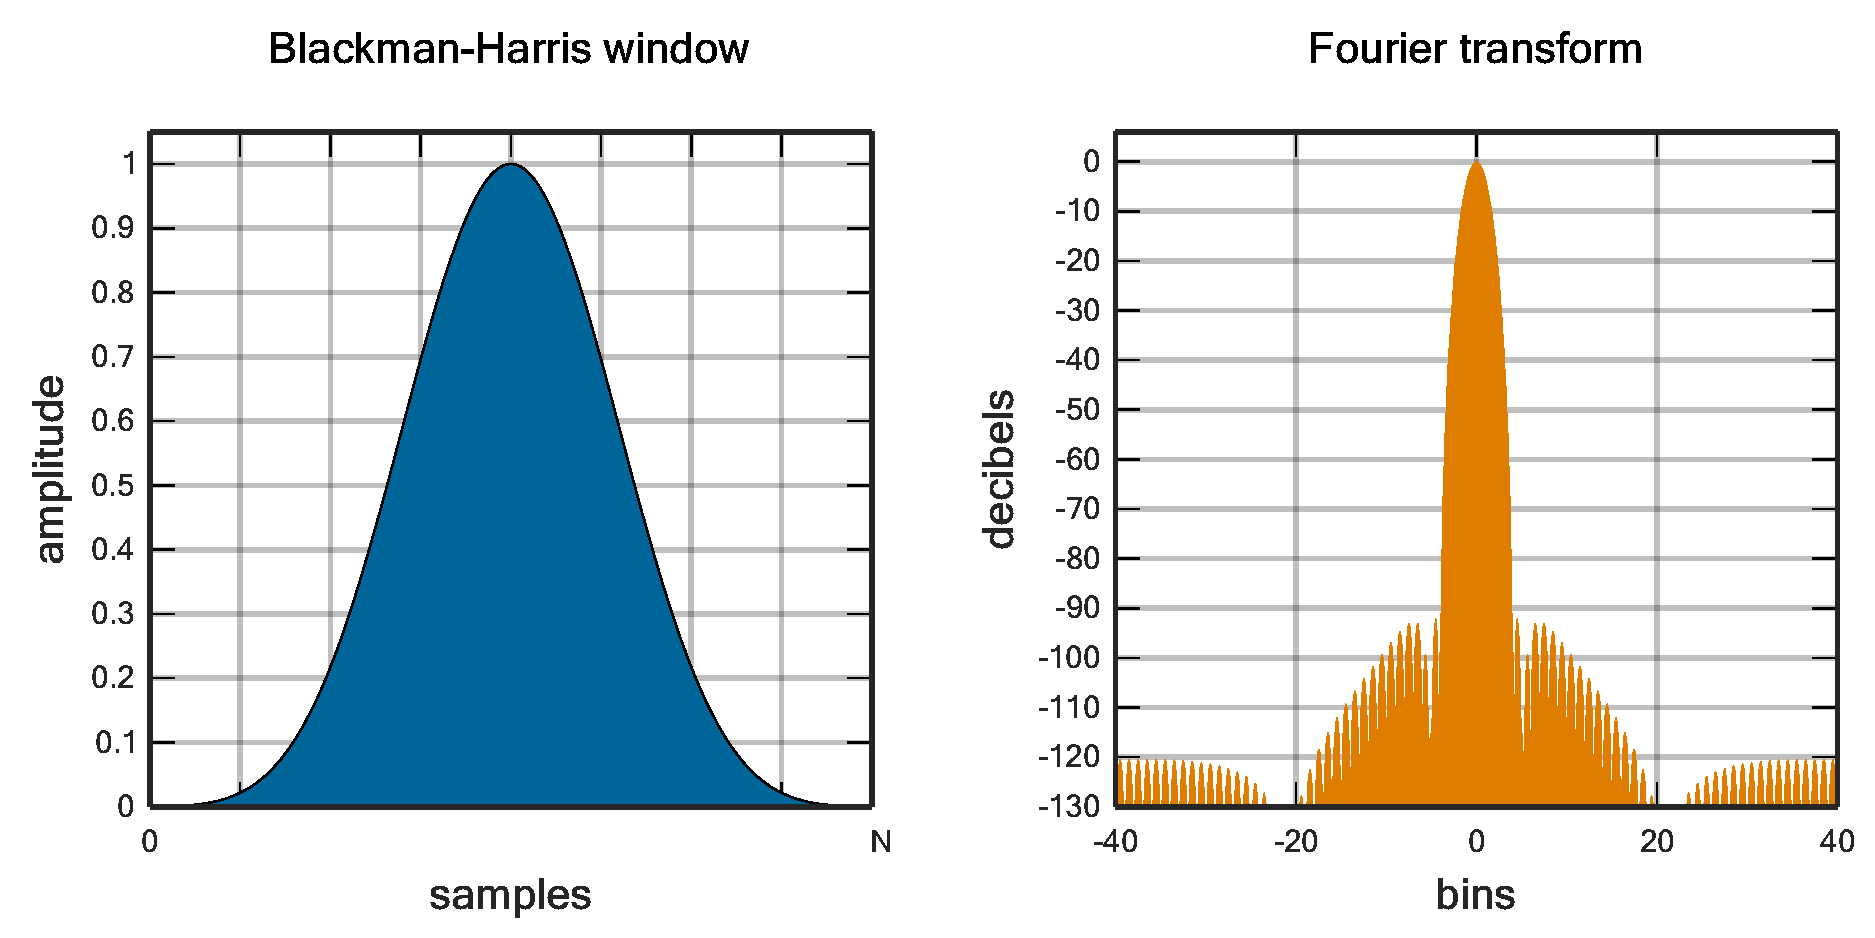
\includegraphics[width=\linewidth]{papers/autotune/sections/fft/images/windows/Blackman-Harris.pdf}
	\end{minipage}

\caption{Verschiedene Fensterfunktionen und deren Beschreibung}\cite{wikipedia:Window}
\label{fig:STFTtab}
\end{figure}



\subsection{Verhalten der STFT}

Wenn man ein Signal mit einer Fensterfunktion Analysiert, zerteilt man das Signal in der Zeitebene vertikal Streifen mit der Breite eines Fensterintervalles. Wendet man nun darauf noch die Fourier-Transformation an wird jeder Streifen in rechtecke aufgeteilt. Die höhe des Rechteckes wird durch die Unschärferelation bestimmt. Daraus folgt bei einem breiteren Streifen ergibt sich eine besser Frequenzauflösung, was jedoch einen schlechtere Zeitauflösung bedeutet. In der Abbildung \ref{fig:stftauf} kann man die grafische Darstellung der Zeit-Frequenz-Auflösung sehen. Bei gleichbleibendem Flächeninhalt der einzelnen Rechtecke ist auf der linken Seite eine feinere Zeitauflösung zu sehen. Wobei Rechts eine bessere Frequenzauflösung aufweist. Dies wird durch die Küpfmüllerschen Unbestimmtheitsrelation welche besagt, dass die Zeitdauer und die Bandbreite eines Signals nicht gleichzeitig beliebig klein werden können. Dies ist eine zur Heisenbergschen Unschärferelation analoge Aussage welche auf die Nachrichtentechnik übernommen werden kann.

\begin{figure}[!ht]
	\centering
	\scalebox{.75}{
	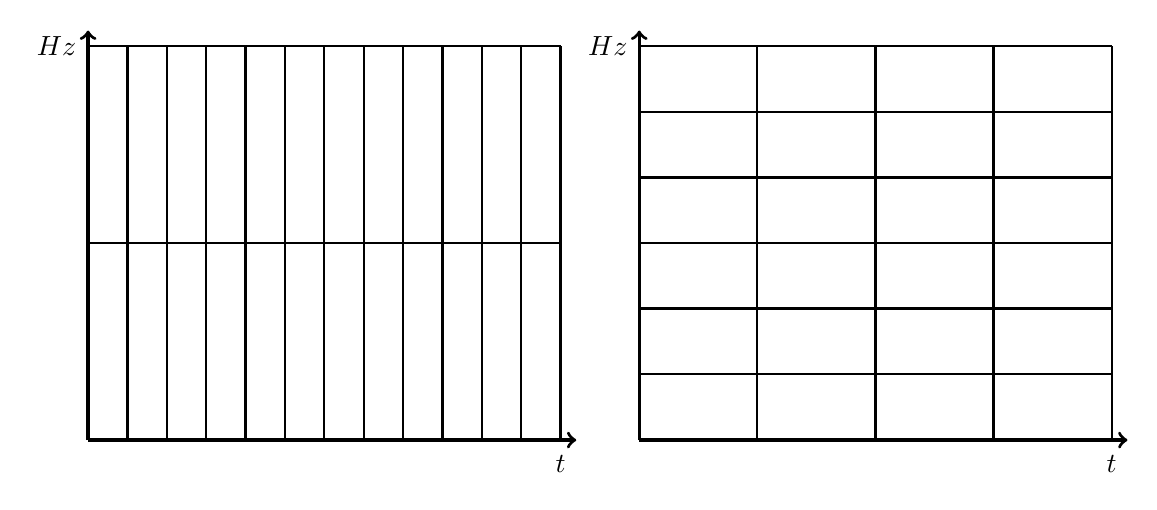
\begin{tikzpicture}
		\draw (6,-5.3) node{$t$};
		\draw (-0.4,0) node{$Hz$};
		\draw[->, very thick] (0,-5)--(0,0.2);
		\draw[->, very thick] (0,-5)--(6.2,-5);
		
		\draw[thick] (0,-0)--(6,-0);
		\draw[thick] (0,-2.5)--(6,-2.5);
		
		\draw[thick] (0.5,-5)--(0.5,0);
		\draw[thick] (1,-5)--(1,0);
		\draw[thick] (1.5,-5)--(1.5,0);
		\draw[thick] (2,-5)--(2,0);
		\draw[thick] (2.5,-5)--(2.5,0);
		\draw[thick] (3,-5)--(3,0);
		\draw[thick] (3.5,-5)--(3.5,0);
		\draw[thick] (4,-5)--(4,0);
		\draw[thick] (4.5,-5)--(4.5,0);
		\draw[thick] (5,-5)--(5,0);
		\draw[thick] (5.5,-5)--(5.5,0);
		\draw[thick] (6,-5)--(6,0);
		
		\draw (13,-5.3) node{$t$};
		\draw (6.6,0) node{$Hz$};
		\draw[->, very thick] (7,-5)--(7,0.2);
		\draw[->, very thick] (7,-5)--(13.2,-5);
		
		\draw[thick] (7,-0)--(13,-0);
		\draw[thick] (7,-0.833)--(13,-0.833);
		\draw[thick] (7,-1.666)--(13,-1.666);
		\draw[thick] (7,-2.499)--(13,-2.499);
		\draw[thick] (7,-3.33)--(13,-3.33);
		\draw[thick] (7,-4.166)--(13,-4.166);
		
		\draw[thick] (8.5,-5)--(8.5,0);
		\draw[thick] (10,-5)--(10,0);
		\draw[thick] (11.5,-5)--(11.5,0);
		\draw[thick] (13,-5)--(13,0);
	\end{tikzpicture}
	}
	\caption{STFT Zeit-Frequenz-Auflösung}\label{fig:stftauf}	
\end{figure}

\begin{figure}[!ht]
	\centering
	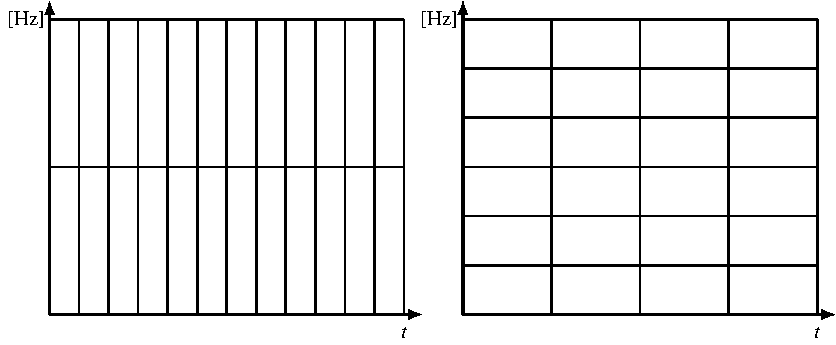
\includegraphics[width=0.7\linewidth]{papers/autotune/sections/fft/images/windows.pdf}
	\caption{STFT Zeit-Frequenz-Auflösung}\label{fig:stftauf}	
\end{figure}





 
Um das zu veranschaulichen  der Unschärferelation betrachten wir einen modulierten Frequensweep von 0 bis 400$[Hz]$. Die Definition der verwendeten Frequenzsweepes $x_{sweep}(t)$ ist folgendermassen:

\begin{equation}
x_{sweep}(t)=\sin \left(2 \pi \int_{0}^{t} f(\tau) \mathrm{d} \tau\right)=\sin \left(2 \pi \int_{0}^{t}\left(f_{0}+k \tau\right) \mathrm{d} \tau\right)=\sin \left(2 \pi\left(f_{0}+\frac{k}{2} t\right) t\right)
\end{equation} 

Der Sweep wird nun mit einem viel langsameren Signal, welches aus einem verschobenen Cosinus besteht, moduliert. Die Defenition des zu Analysierende Signales $f(t)$ lautet dementsprechend:
\begin{equation}
f(t)= (-0.5\cdot \cos(nt)+0.5)\cdot x(t)=(-0.5\cdot \cos(nt)+0.5)\cdot \sin \left(2 \pi \int_{0}^{t} f(\tau) \mathrm{d} \tau\right)
\end{equation} \label{eq:sin-sweep}
wobei $n$ die Anzahl von Perioden des Cosinus in einer Zeit von $2\pi$ ist. Danach wurde $f(t)$ mit dem STFT Verfahren analysiert. Insgesamt wurde $f(t)$ vier mal analysiert. Jede Analyse wurde mit der Blackman Fensterfunktion durchgeführt jedoch wurden die Fenster in ihrer Breite verändert. Diese Veränderung trägt zu dem Verständnis der Unschärferelation bei. Die verwendete Blackmanfunktion ist in der Tabelle \ref{tab:STFTtab} definiert.\\

In der Grafik \ref{fig:STFT} kann nun diese Unschärferaltion beobachtet werden. Die Unschärfe wird gut erkennbar wenn man ein beliebiges Signal mit zeitlich verschieden langen Fenstern Analysiert. Wobei bei diskreten werten dies direkt in anzahl Samples pro Fenster gesehen werden muss.\\



\begin{figure}[!ht]
	\centering
	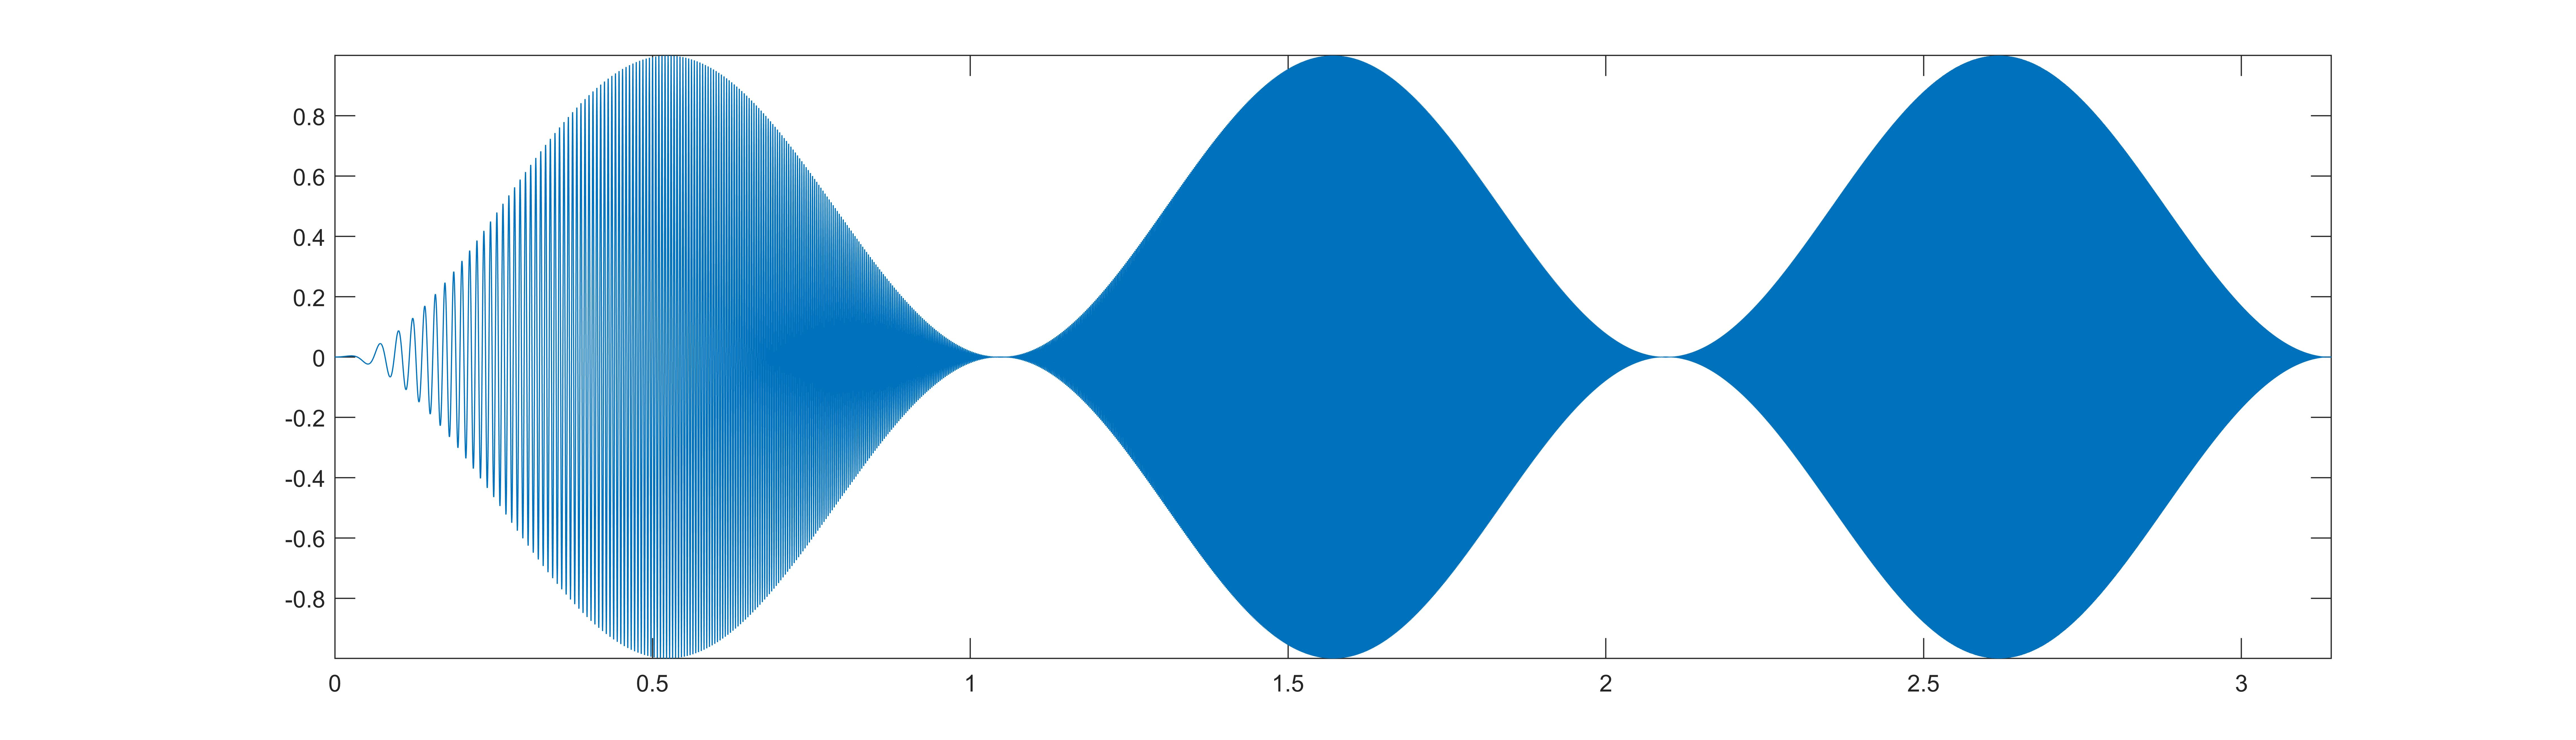
\includegraphics[width=\linewidth]{papers/autotune/sections/fft/signal.jpg}
	\captionof{figure}{Sweep Signal 0-400$Hz$}\label{fig:stftsig}
	\begin{tabularx}{\columnwidth}{XX}
		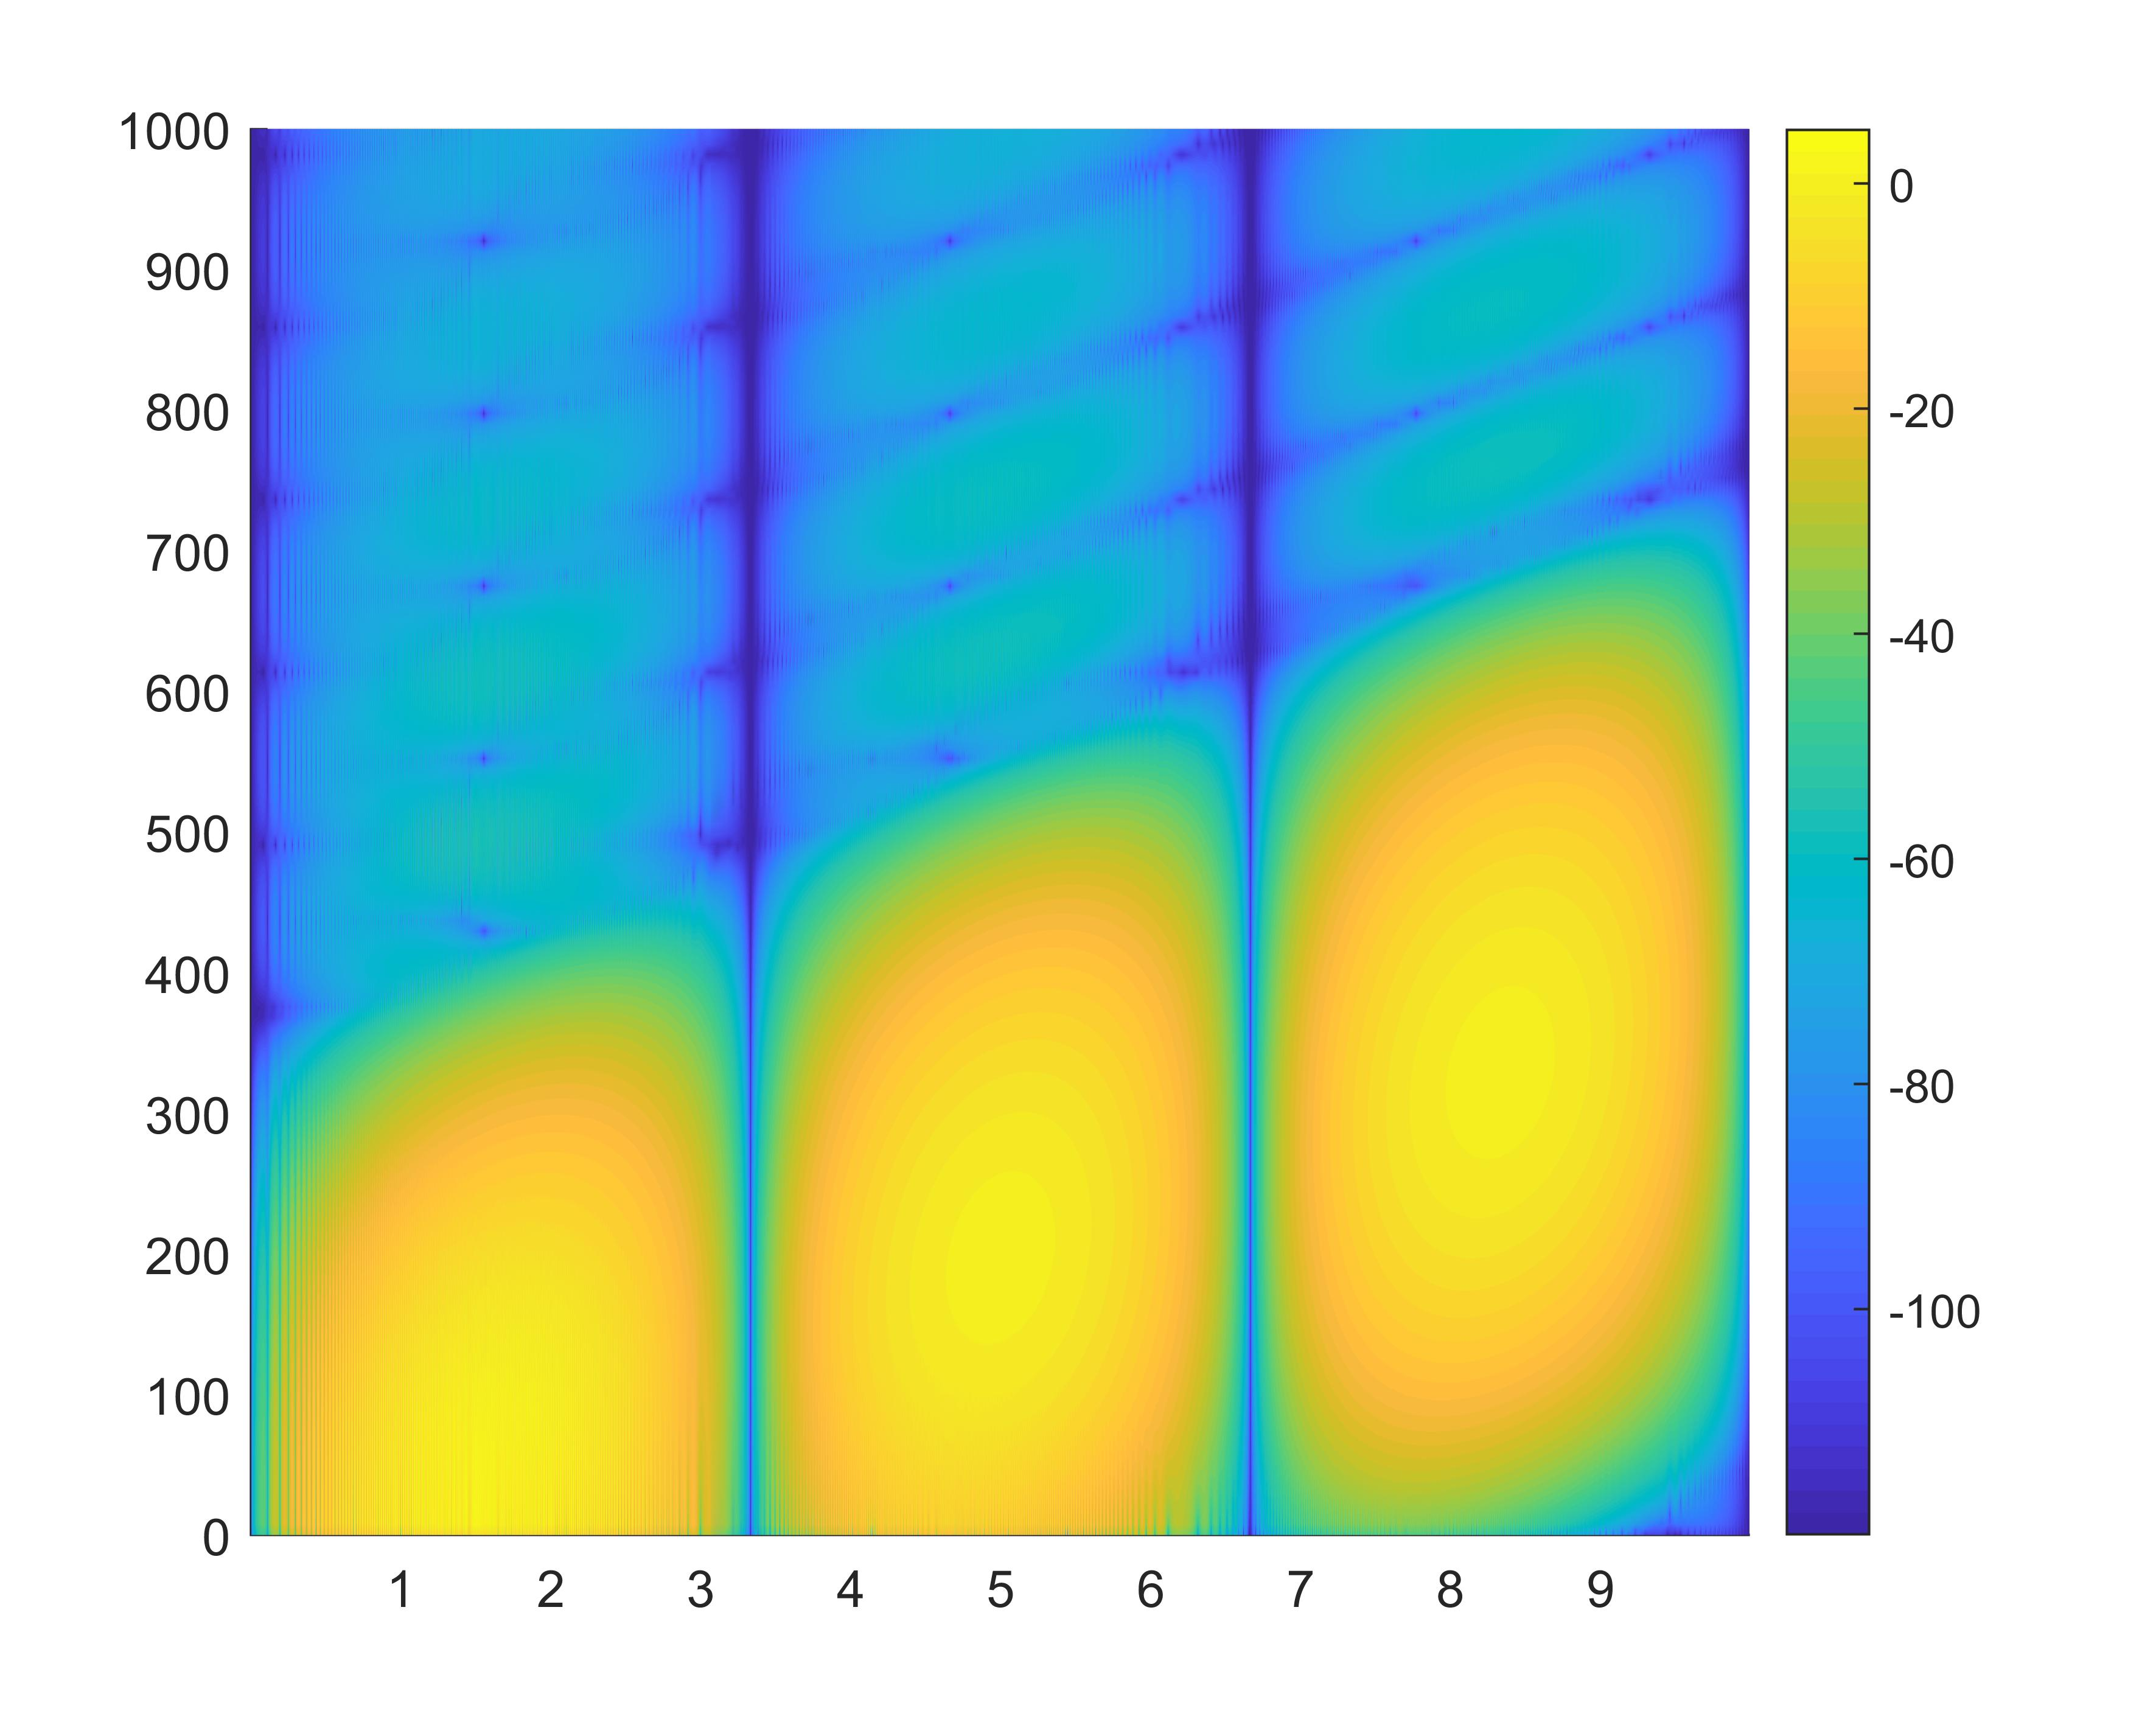
\includegraphics[width=\linewidth]{papers/autotune/sections/fft/stft256.jpg}
		\captionof{figure}{256 Sample Fenster}\label{fig:stft256}
		&   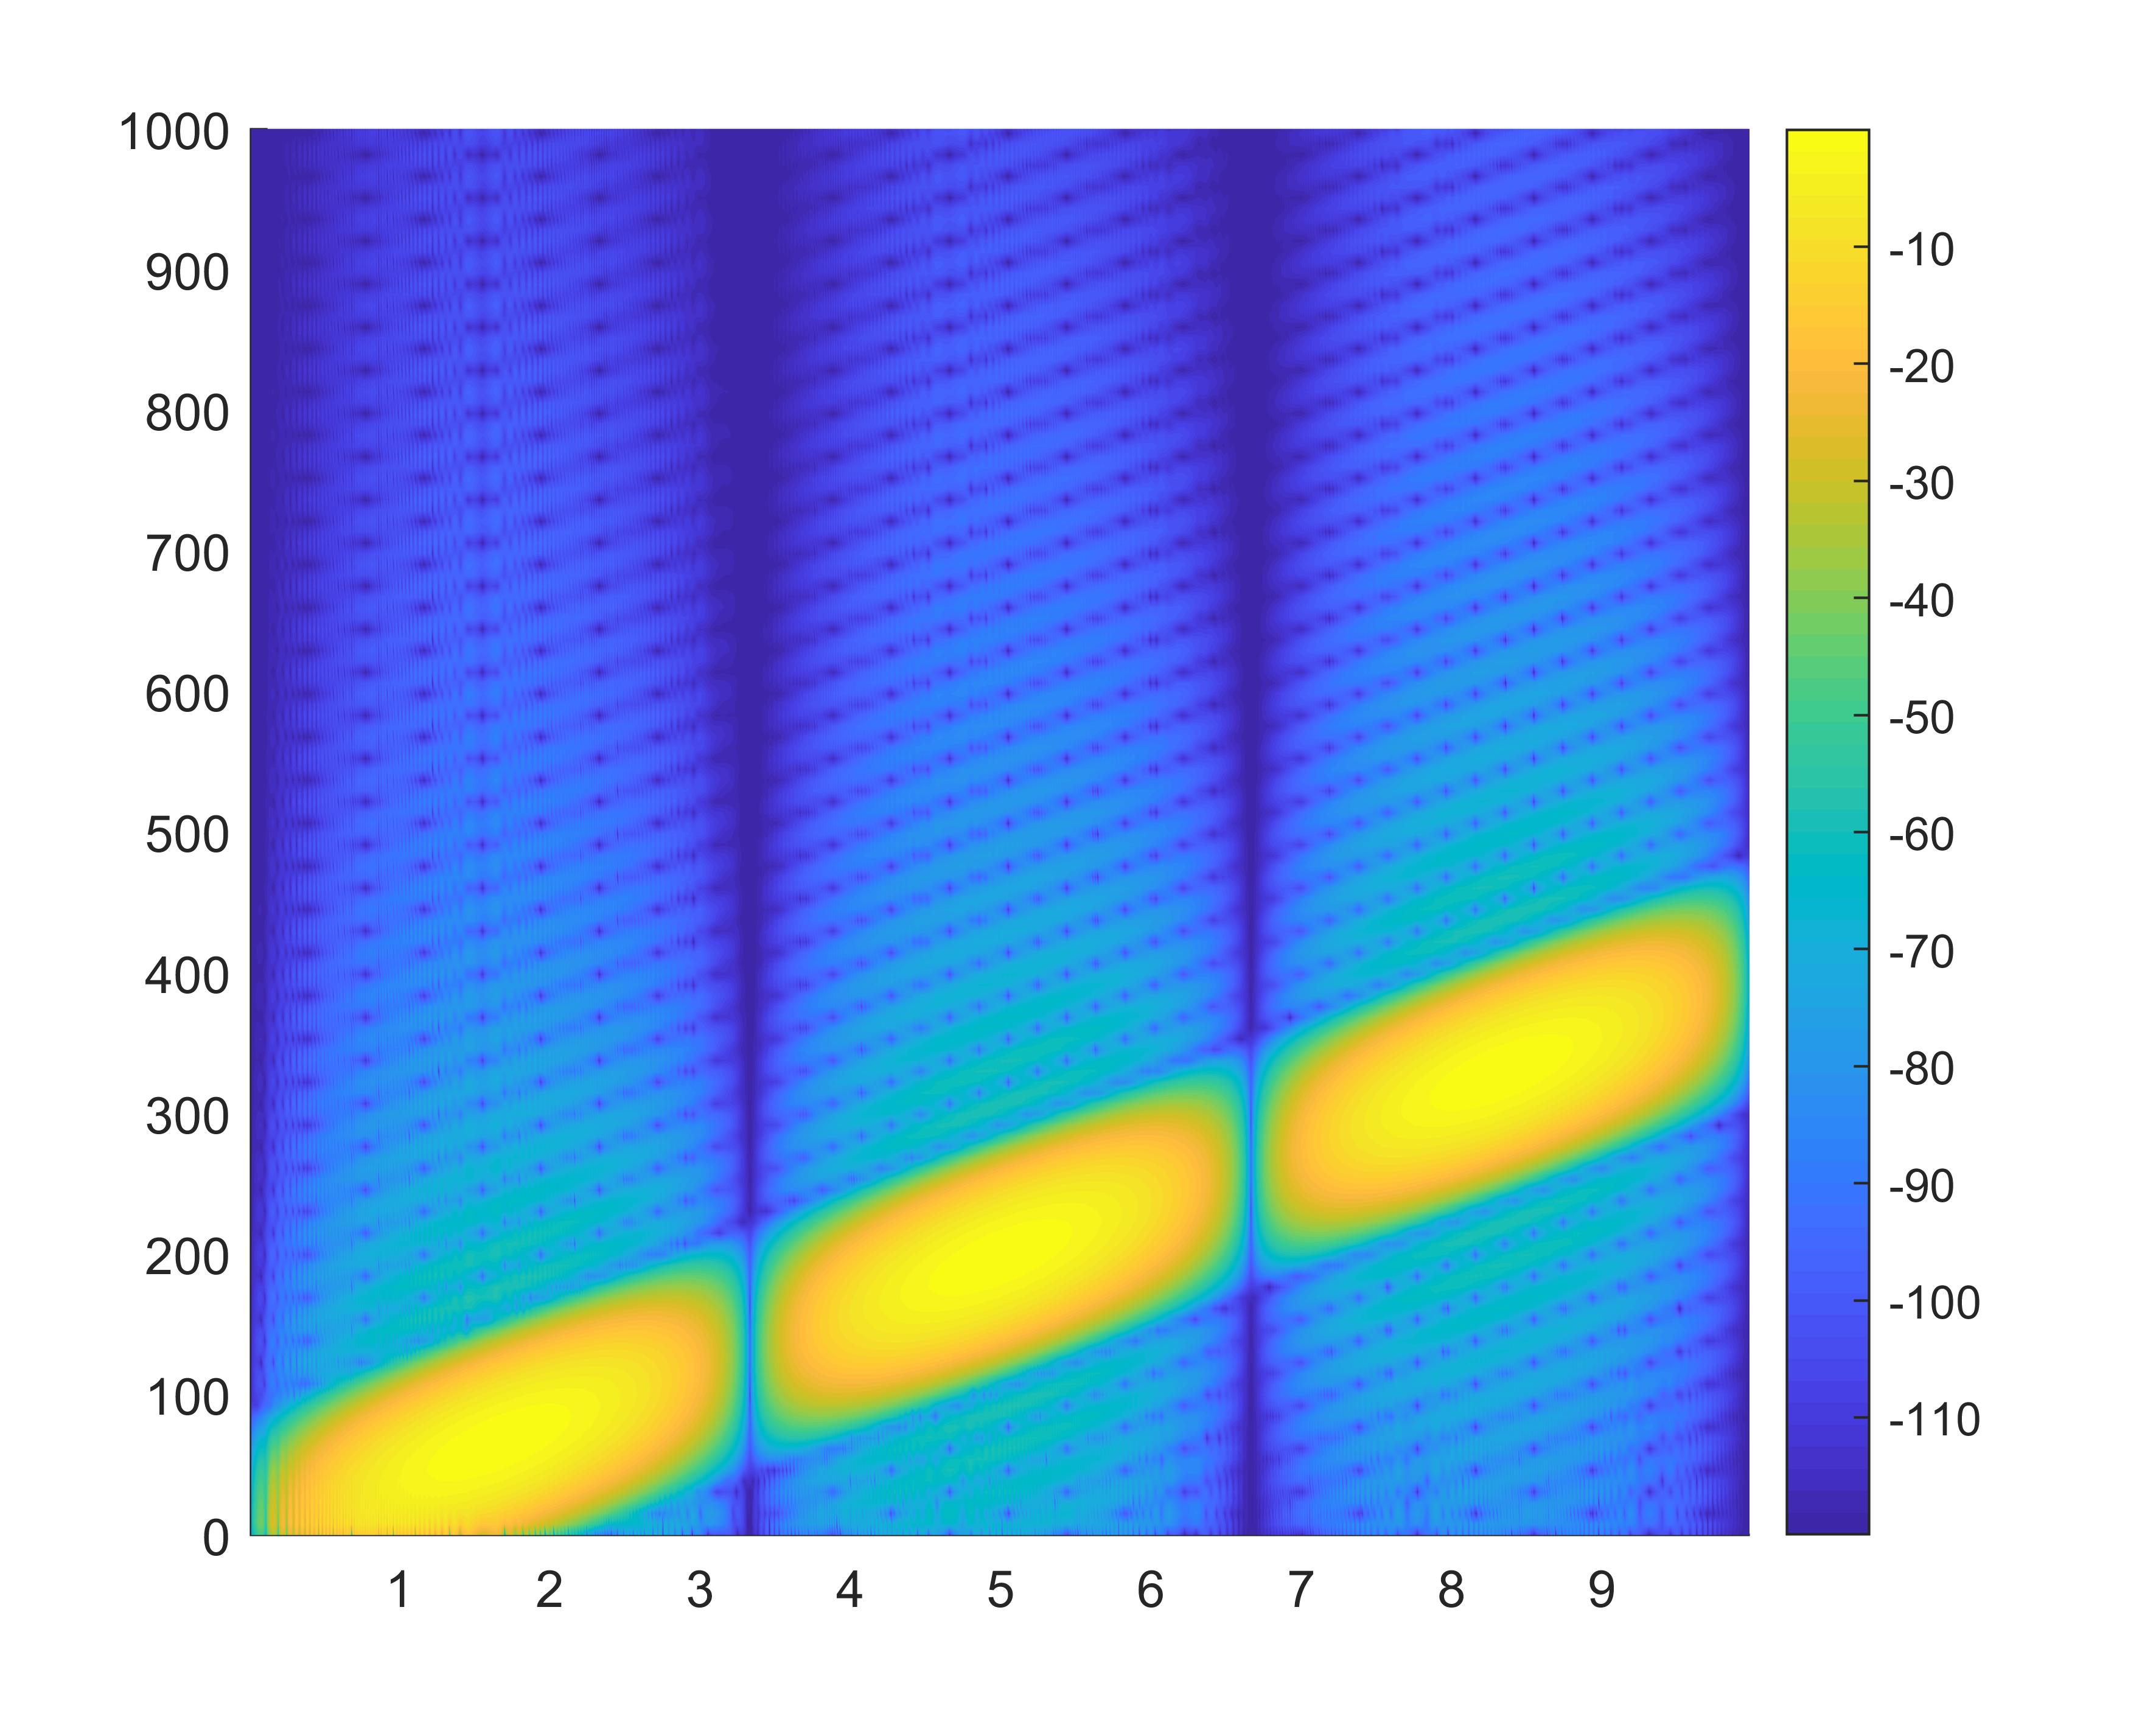
\includegraphics[width=\linewidth]{papers/autotune/sections/fft/stft1024.jpg}   
		\captionof{figure}{1024 Sample Fenster}\label{fig:stft1024}              \\    
		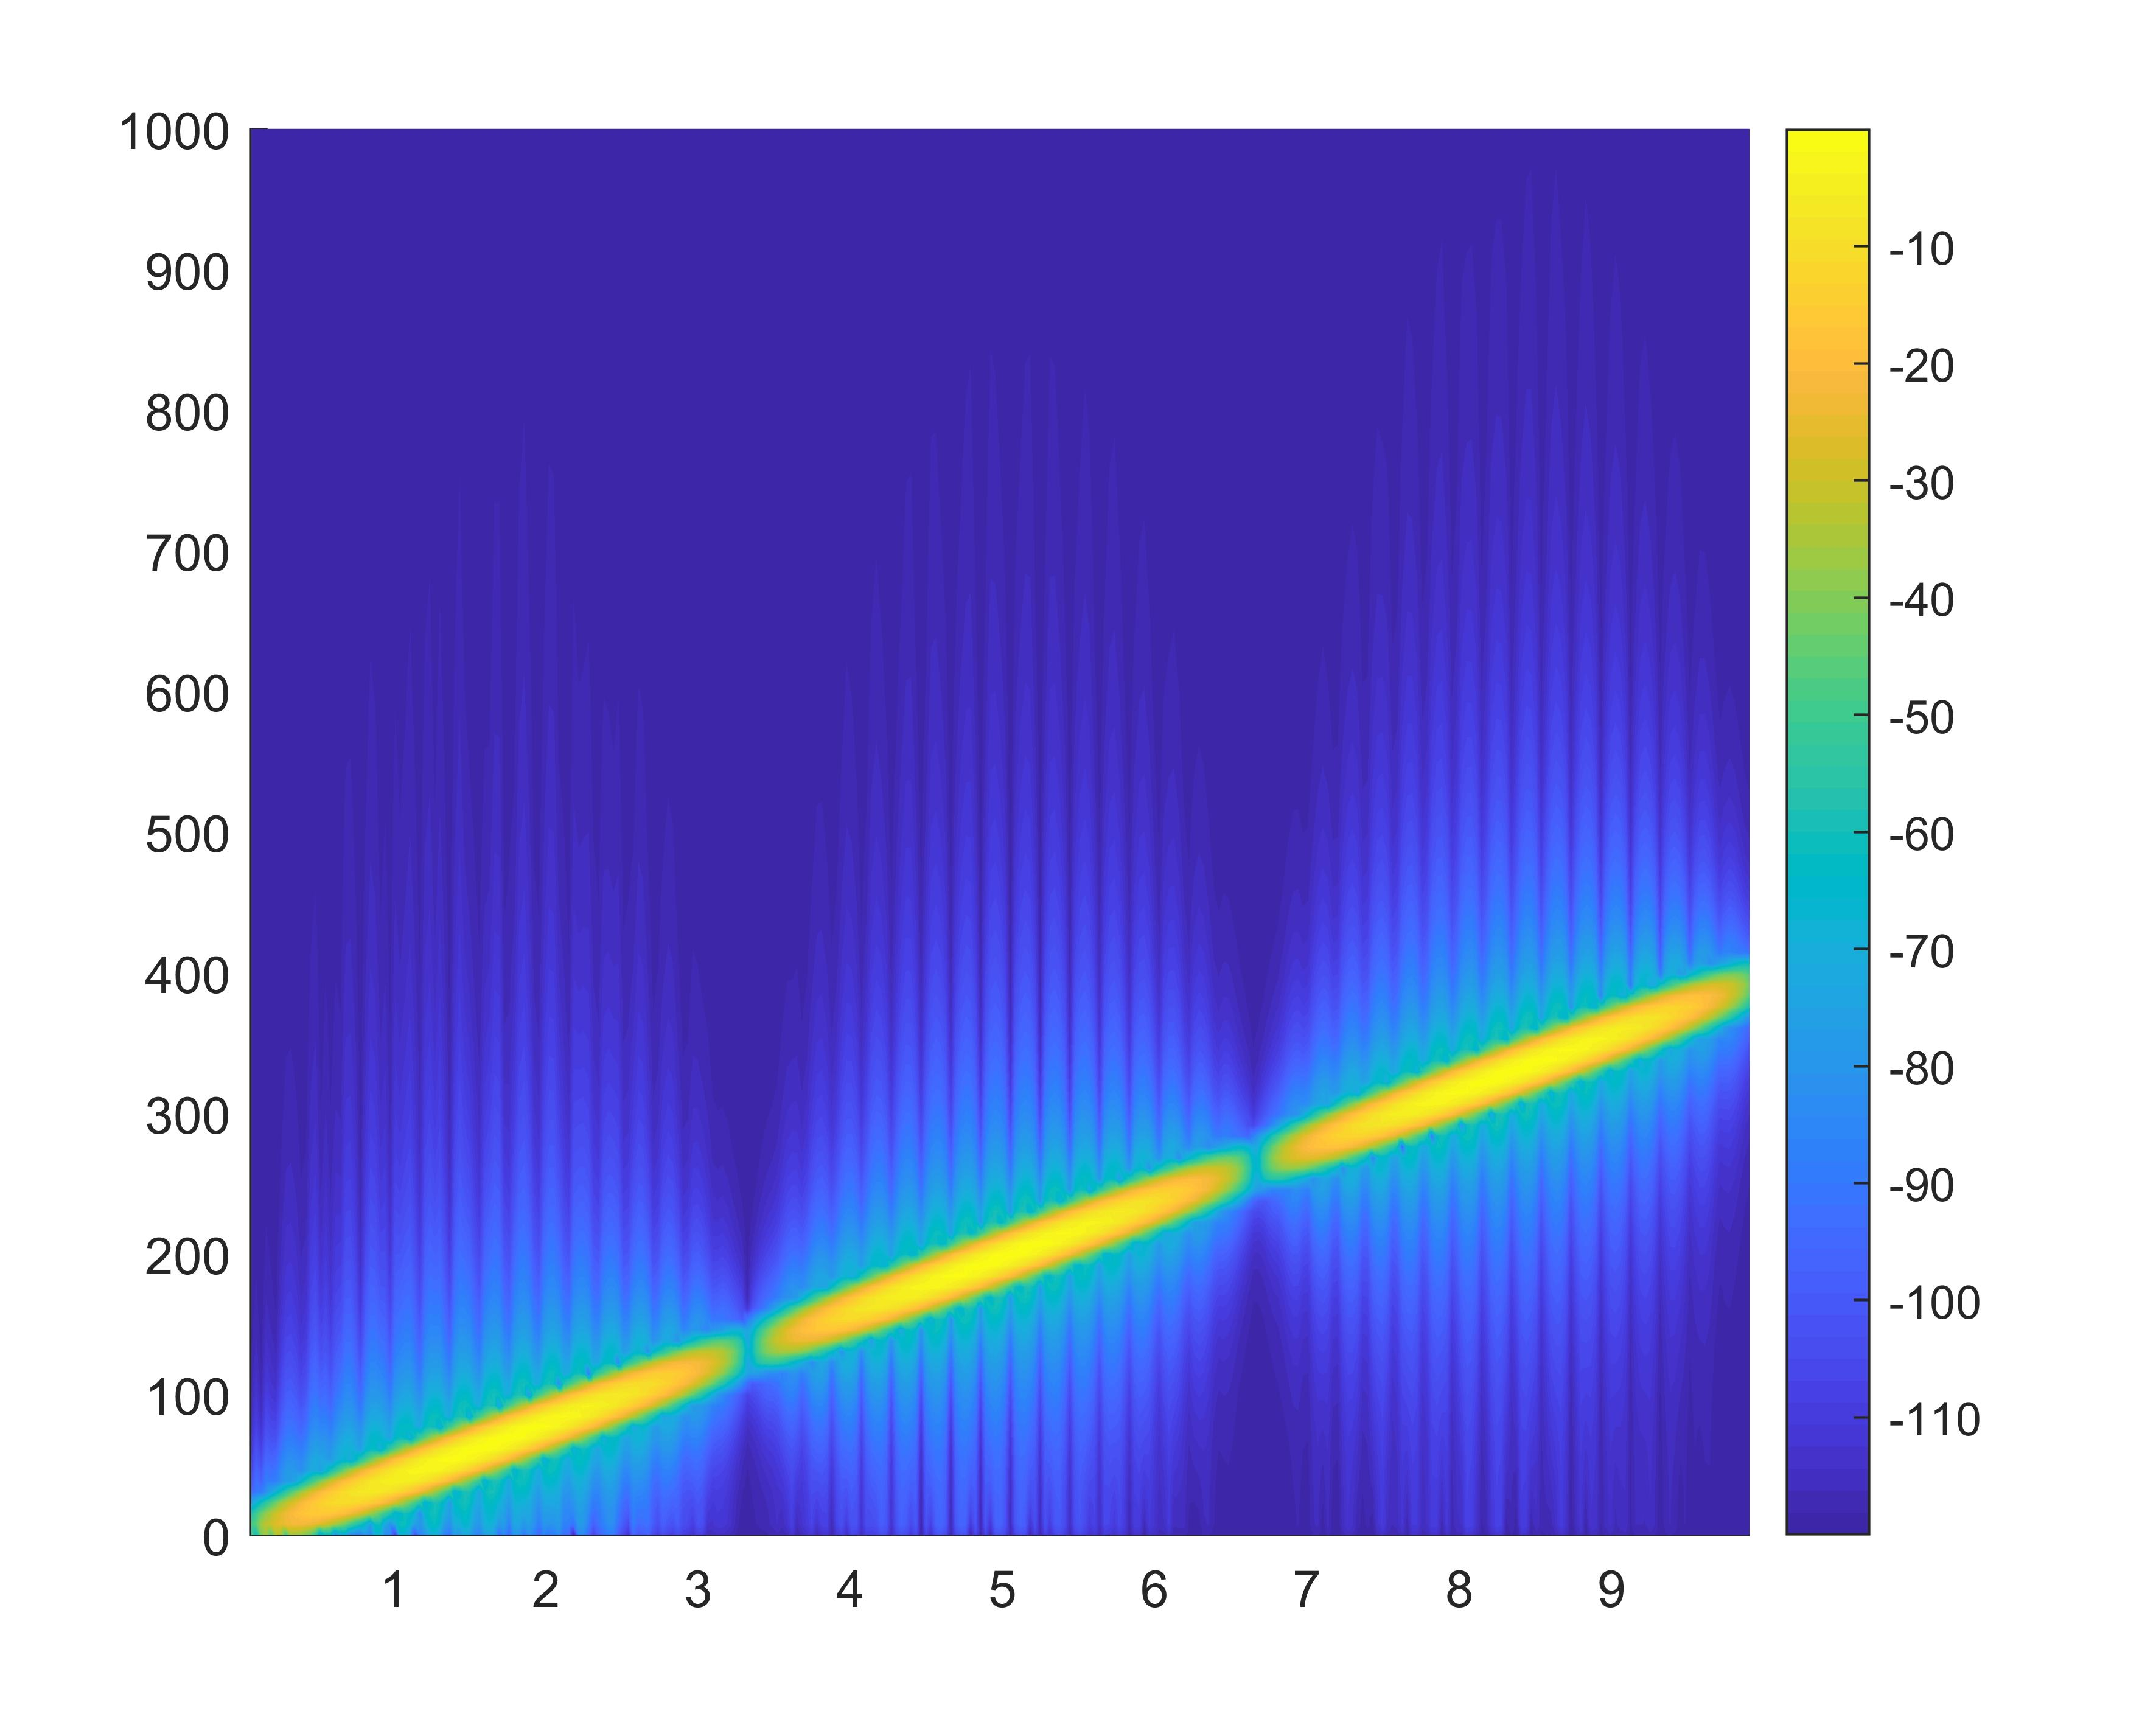
\includegraphics[width=\linewidth]{papers/autotune/sections/fft/stft4096.jpg}
		\captionof{figure}{4096 Sample Fenster}\label{fig:stft4096}
		&   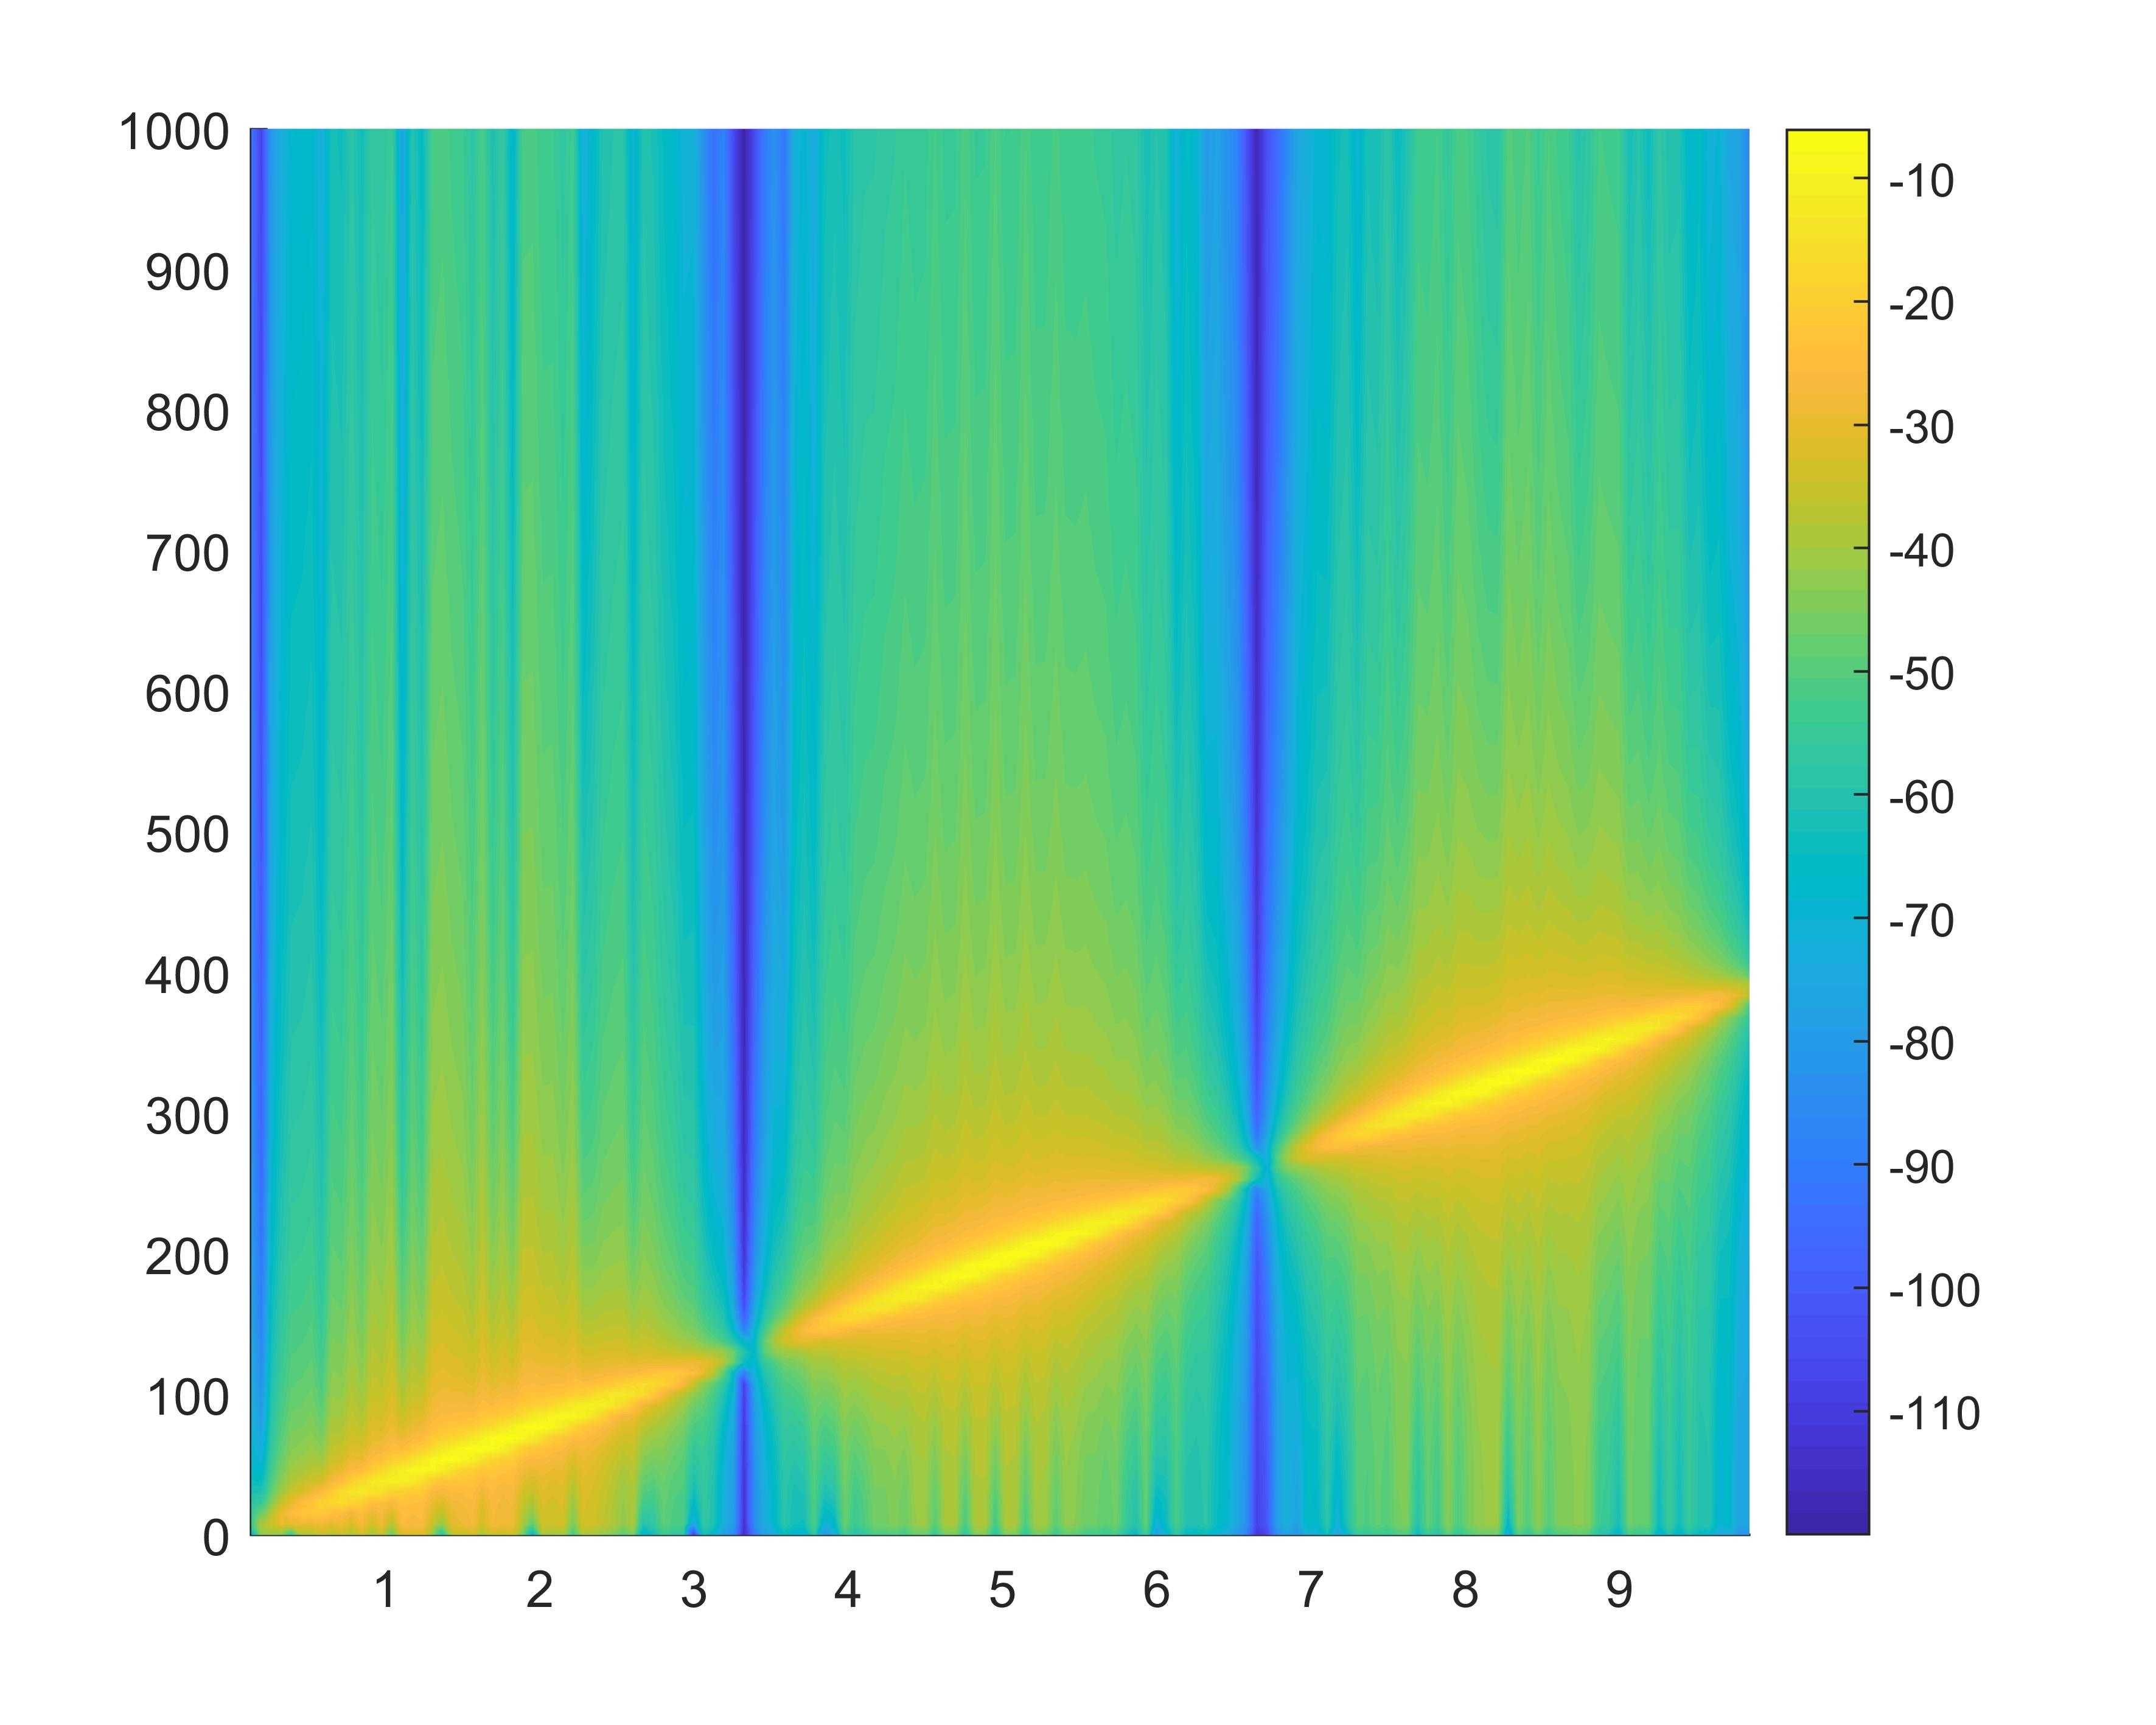
\includegraphics[width=\linewidth]{papers/autotune/sections/fft/stft8192.jpg}   
		\captionof{figure}{8192 Sample Fenster}\label{fig:stft8192}              \\           
	\end{tabularx}
	
	\caption{STFT}
	\label{fig:STFT}
\end{figure}%


Wie man bei der Abbildung \ref{fig:stft256} gleich sieht ist die Streuung noch ernorm. Mann kann nur sehr grob wahrnehmen welche Frequenzen vorhanden sind. Dafür ist die Zeitliche Auflösung sehr gut mit einer scharfen Kante beim Nullpunkt. \\

Betrachtet man nun die Abbildung \ref{fig:stft1024} sind die Frequenzen schon viel deutlicher zu erkennen als bei einem Sampling von 256. Dafür wird in der Zeitlichen Auflösung ein wenig eingebüsst.\\

Das beste Bild ist bei 4096 Samples in der Abbildung \ref{fig:stft4096} zu sehen. Die Zeitliche abgrenzung verschwimmt ein wenig. Dafür ist die Frequenz deutlich ersichtlich.\\

In der Letzten Abbildung \ref{fig:stft8192} ist die zeit so langsam das die tiefen Frequenzen des Modultionssignal wieder einfluss nehmen auf das Spektogramm. Dies verfälscht das Resultat welches dann weniger brauchbar sein kann bei praktischen Auswertungen bei der die Modulationsfrequenz nicht so eine wichtige Rolle spielt.\\







\newpage

\section{Frequenzanalyse mit Wavelets}
\rhead{Frequenzanalyse mit Wavelets}

In diesem Abschnitt wird die stetige und diskrete Wavelet-Transformation betrachtet. Dabei soll ein überblick über die Vor- und Nachteile zur Frequenz-Zeit-Spektrum analyse geschaffen werden. 



\subsection{Stetige Wavelet-Transformation} 
Im Kapitel \ref{chapter:cwt} wurde die Theorie der stetigen Wavelet-Transformation behandelt. In dieser Theorie haben wir gesehen das wir mit der Stetigen Wavelet-Transformation ein Zeit-Frequenz Analyse machen kann und gut interpretierbare Egebnisse erhält. Der Nachteil bei der cwt ist jedoch die grosse Redundanz. Diese Redundanz spiegelt sich in der Analysedauer wieder. Welsche schon bei simplen Datensätzen mehrere Sekunden dauern kann. Weshalb sie für eine realtime Applikation nicht geeignet ist.\\
Um dennoch die zu zeigen welche vorteile eine cwt bringen kann wurde noch einmal der Frequenzsweep \ref{fig:stftsig} mit einem Komplexen Gauss Wavelet Analysiert. Das komplexe Gauss-Wavelet ist wie folgt definiert:
\begin{equation}
\psi(t)=C \cdot e^{-it} e^{-t^{2}}
\label{eq:cgau}
\end{equation}
Wobei $C$ eine Konstante ist. Das komplexe Gauss Wavelet wird in der folgenden Analyse in der achten Ableitung verwendet. In der Python Library wird dies $\texttt{cgau}N$ benennt wobei N für die häufigkeit der Ableitungen der Wavletfunktion steht.\\

Die Analyse wurde mit der Python Library pywt durchgeführt welche schon eine komplette cwt-Funktion bereitstellt. In der folgenden Abbildung \ref{fig:python-cwt} ist der wesentliche Ausschnitt aus dem Python Code dargestellt mit dem die cwt Analyse jeweils erstellt wurde. Da es sich um ein komplexes Wavelet handelt, wurde zur besseren veranschaulichung, die Absolutwerte der Analyse zur illustration verwendet.\\

\begin{figure}
	\centering
	\lstinputlisting[language=Python,firstline=9,lastline=26,numbers=left,style = Python]{papers/autotune/sections/frequenzanalyse/code/cwt.py}
	\caption{Python cwt Beispiel}
	\label{fig:python-cwt}
\end{figure}

Das Ergebnis der cwt ist in der Grafik \ref{fig:STFTCWT} ersichtlich. Dabei stehen sich eine STFT und cwt gegenüber. Dringend ist zu betrachten, dass dieser Vergleich auf keinsterweise eine allgemeingültige Aussage über diese zwei Arten der Zeit-Frequenz Analyse sein soll. Sondern mehr eine gegenüberstellung zur betrachtung von unterschieden. 

\begin{figure}[!ht]
	\centering
	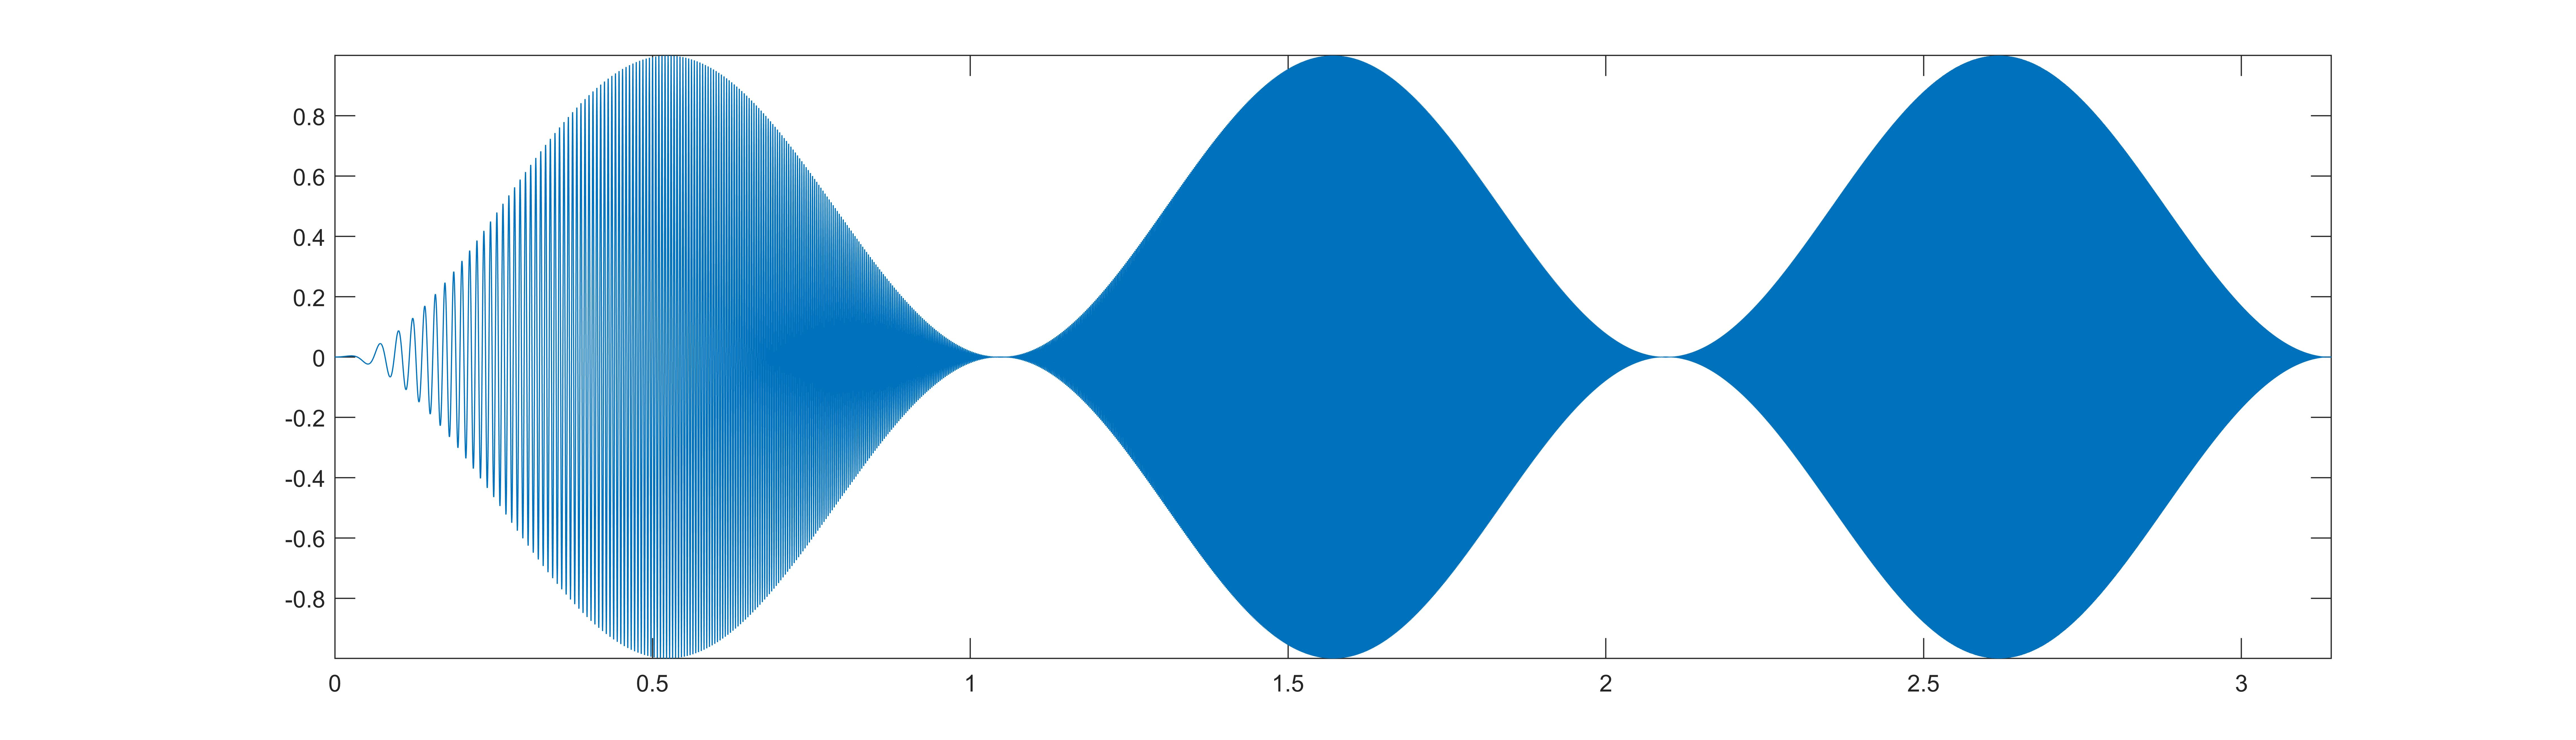
\includegraphics[width=\linewidth]{papers/autotune/sections/fft/signal.jpg}
	\captionof{figure}{Sweep Signal 0-400$Hz$}\label{fig:stftsig}
	\begin{tabularx}{\columnwidth}{XX}
		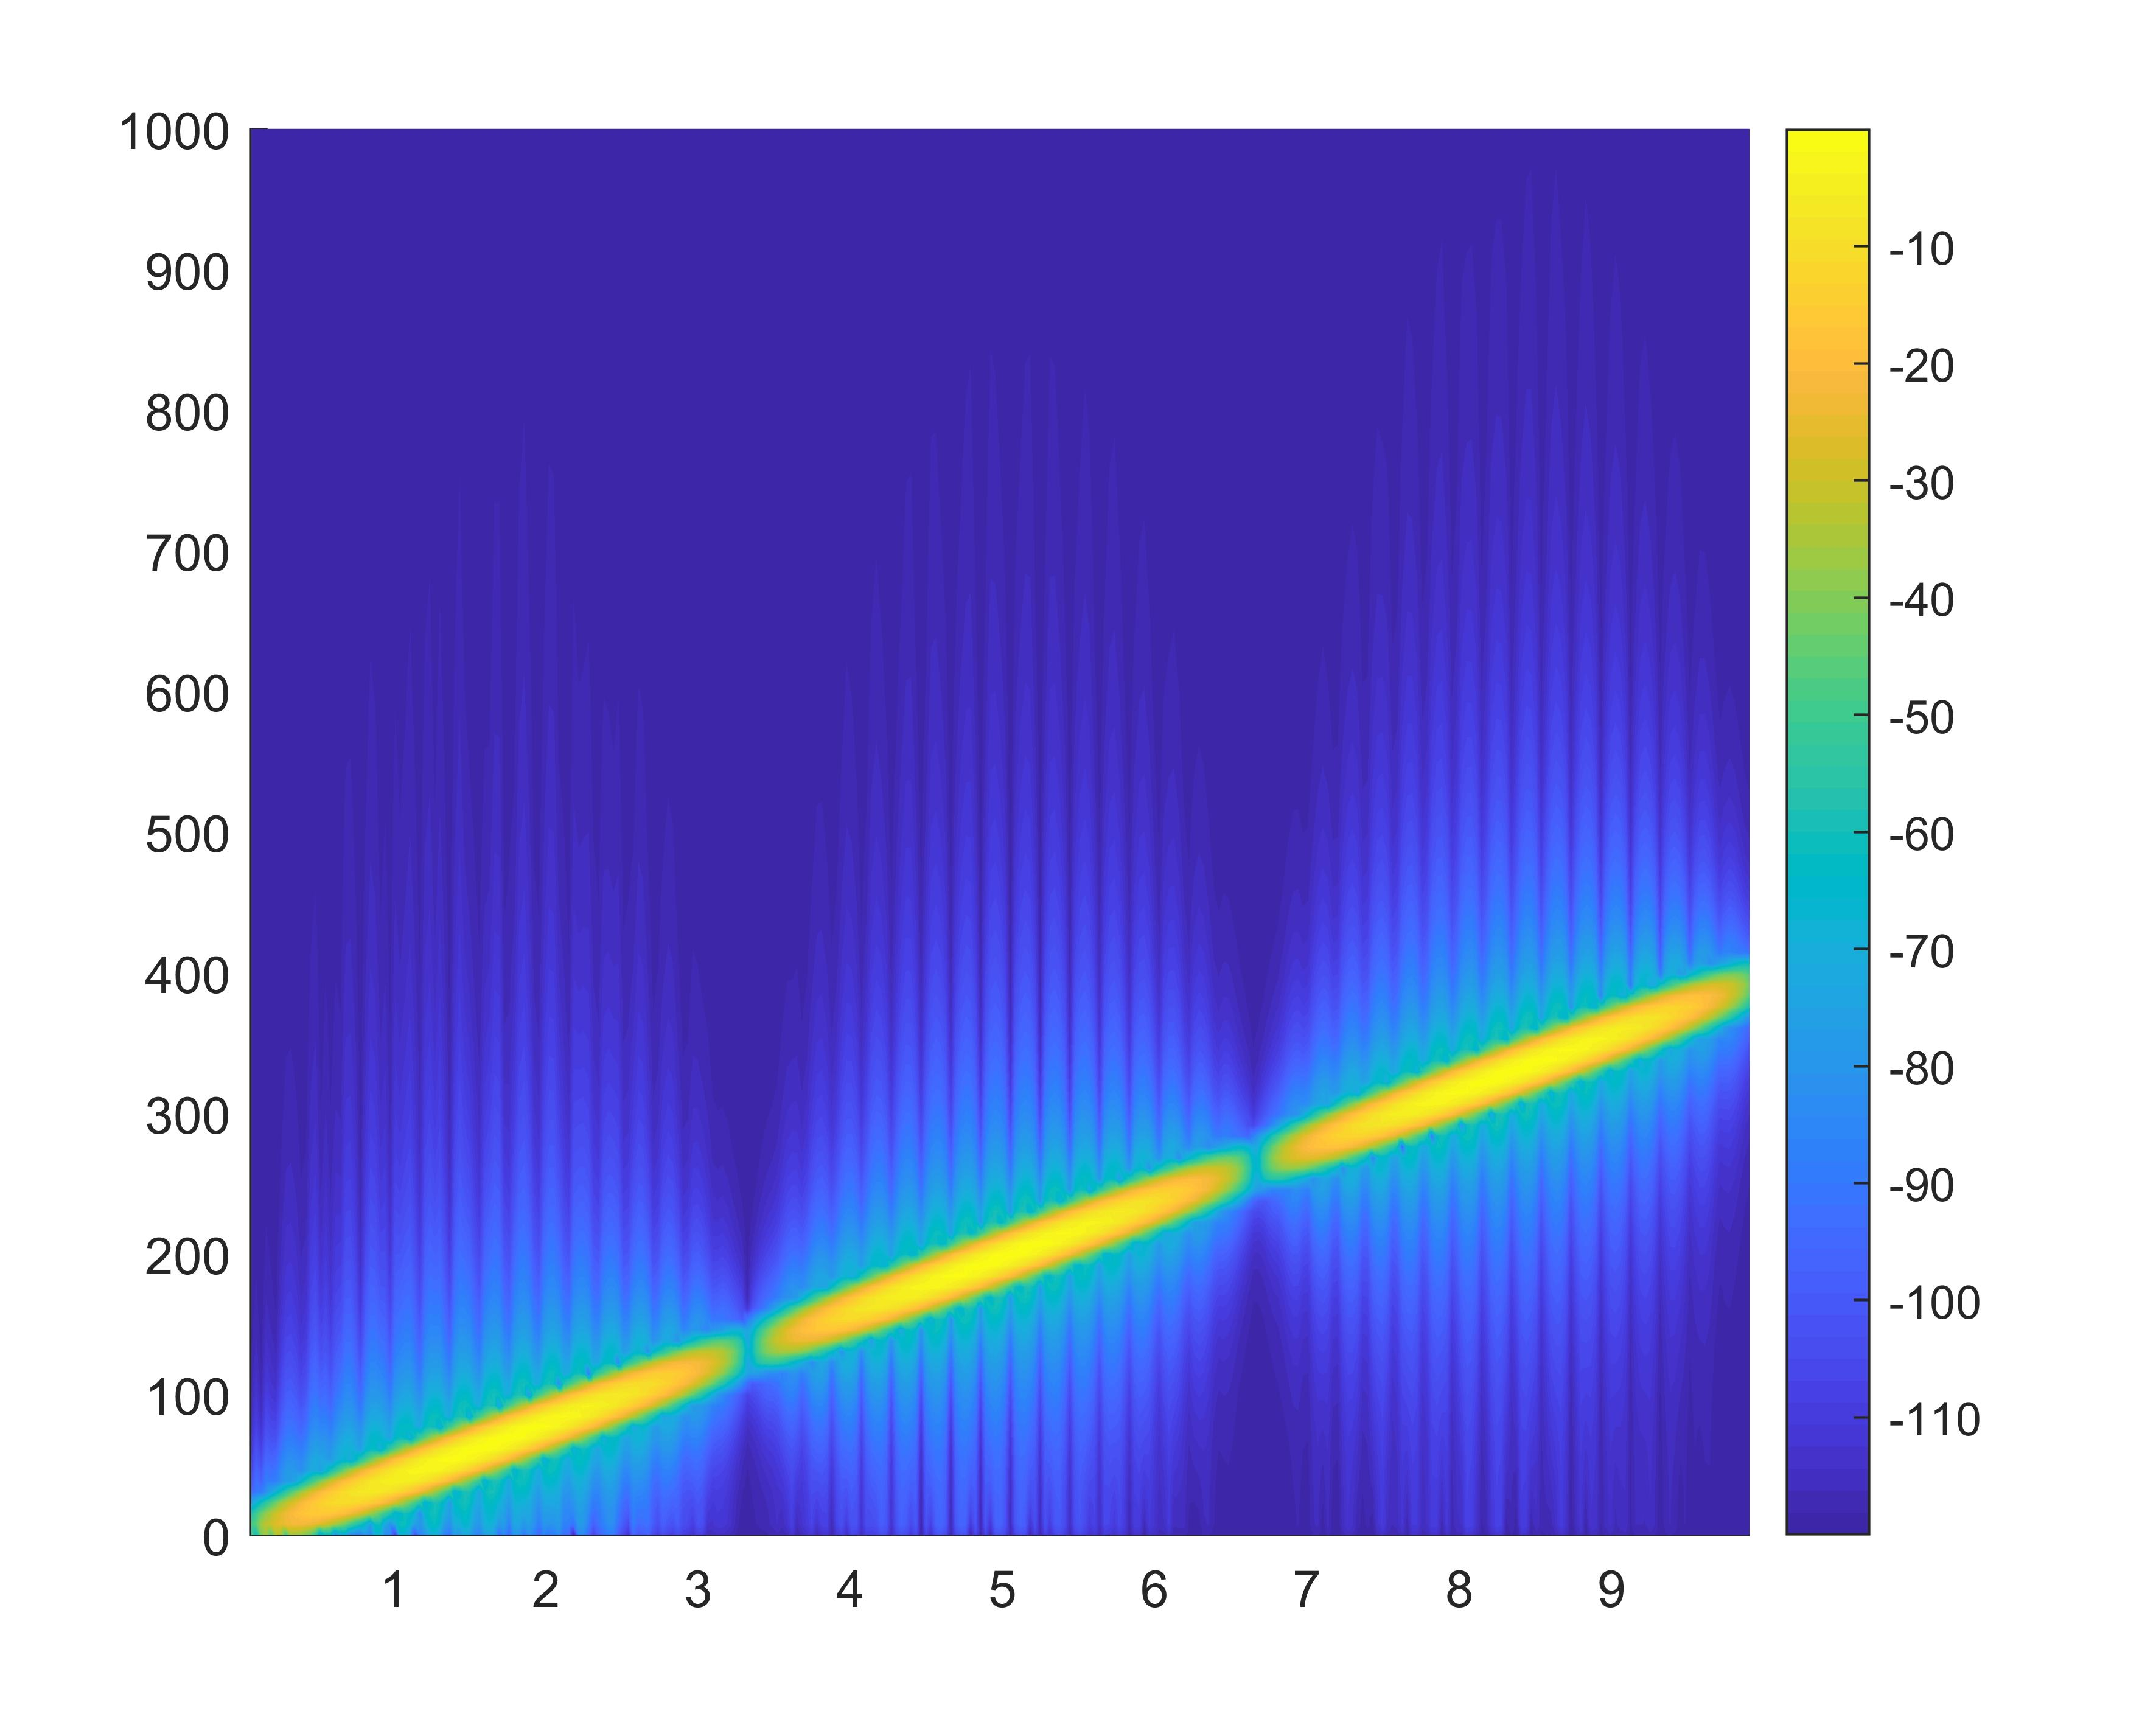
\includegraphics[width=\linewidth]{papers/autotune/sections/fft/stft4096.jpg}
		\captionof{figure}{STFT Blackman mit 4096 Sample Fenster}\label{fig:stft256}
		&   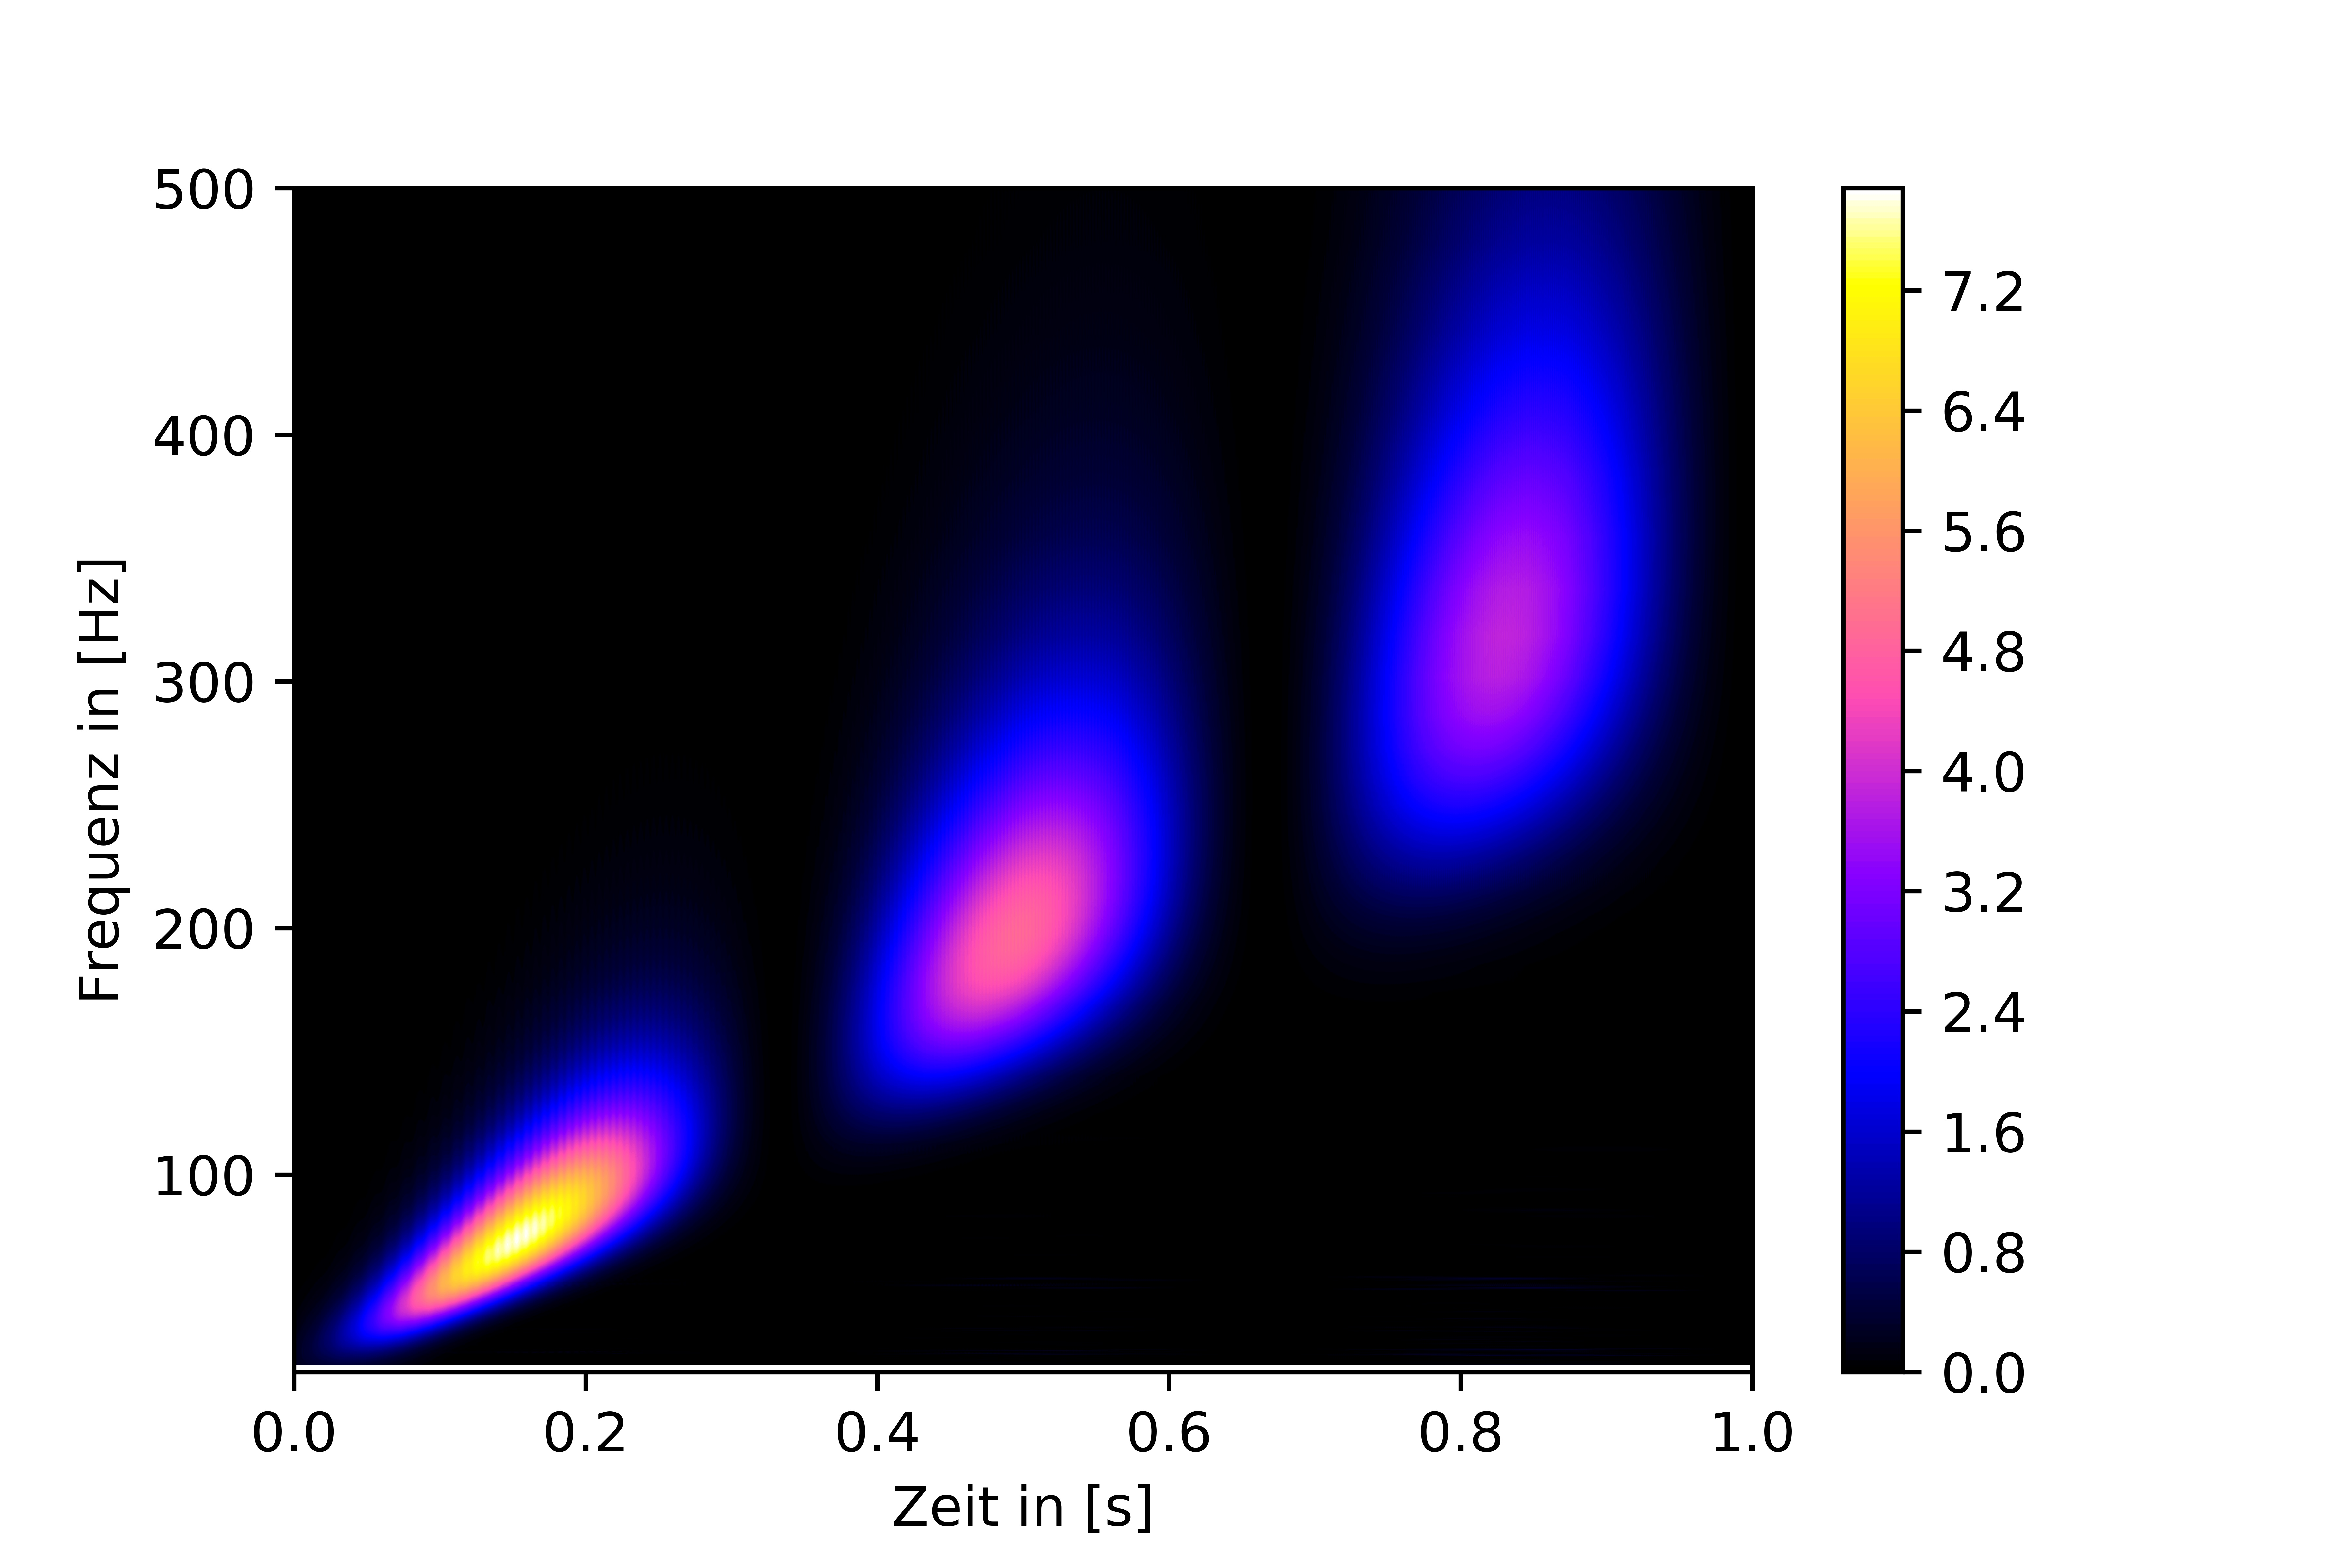
\includegraphics[width=1.24\linewidth]{papers/autotune/sections/frequenzanalyse/images/sinsweep.jpg}   
		\captionof{figure}{Komplex Gauss 8 \ref{eq:cgau} Cwt Analyse des Frequensweeps}\label{fig:cwtsweep}         
	\end{tabularx}
	\caption{figure}{Vergleich zwischen STFT und der CWT}
	\label{fig:STFTCWT}
\end{figure}%


\subsection{Diskrete Wavelet-Transformation}
Im Kapitel \ref{chapter:haar-wavelet} wurde mit dem Haarwavelet welche Problematik eine nicht stetige Wavelet-Transformation verursachen kann. Um eine diskrete Wavelet-Transformation zu berechnen bietet sich der schnelle Multiskalenanalyse Algorhytmus an. Für die analyse ist jedoch die Erkenntnis, dass nur Frequenzen verwendet werden die $2^n$-fache einer Grundfrequenz sind, ausschlaggebend. Die Analyse kann also nur Oktaven unterscheiden, während Töne auf einer Tonleiter Frequenzverhältnisse von $\sqrt[12]{2}$ haben. Wir können also mit einer normalen Multiskalenanalyse nicht einzelne Töne eines Signales unterscheiden. Dennoch können wir gewisse Vorteile nutzen wie die Fensterung des Signales. Die Mutiskalenanalyse hat eine $2^n$-fache Fensterungseigenschaft. In der folgenden Grafik\ref{fig:faauf} ist die Zeit-Frequenz-Fensterung der Multiskalenanalyse neben der STFT Fensterung aufgezeigt.   

\begin{figure}[!ht]
	\centering
	\scalebox{.75}{
		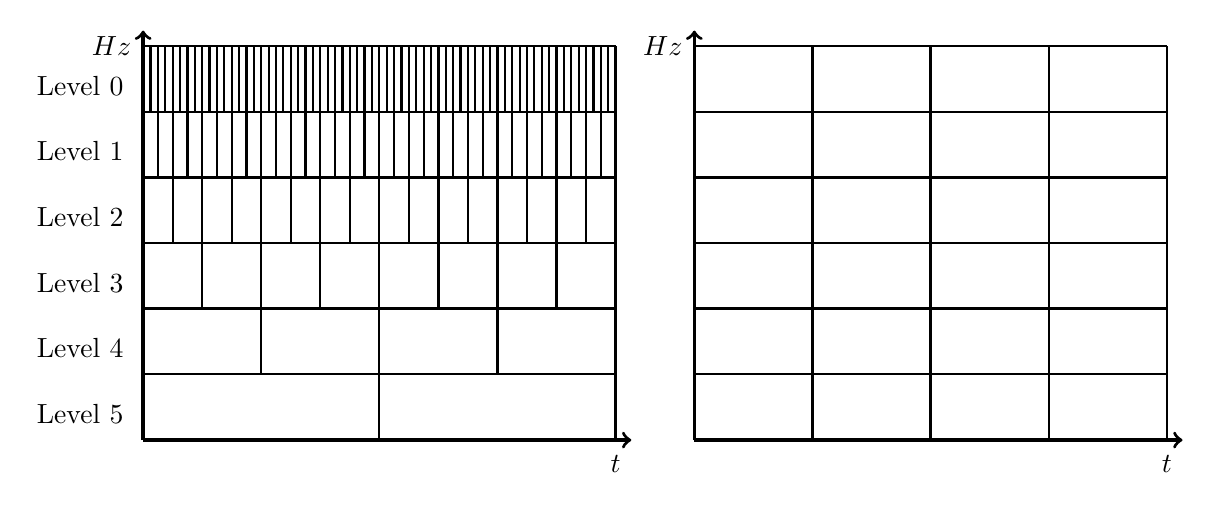
\begin{tikzpicture}
		\draw (6,-5.3) node{$t$};
		\draw (-0.4,0) node{$Hz$};
		
		\draw (-0.8,-0.5) node{Level 0};
		\draw (-0.8,-1.333) node{Level 1};
		\draw (-0.8,-2.166) node{Level 2};
		\draw (-0.8,-2.999) node{Level 3};
		\draw (-0.8,-3.832) node{Level 4};
		\draw (-0.8,-4.665) node{Level 5};
		
		
		\draw[->, very thick] (0,-5)--(0,0.2);
		\draw[->, very thick] (0,-5)--(6.2,-5);
		
		\draw[thick] (0,-0)--(6,-0);
		\draw[thick] (0,-0.833)--(6,-0.833);
		\draw[thick] (0,-1.666)--(6,-1.666);
		\draw[thick] (0,-2.499)--(6,-2.499);
		\draw[thick] (0,-3.33)--(6,-3.33);
		\draw[thick] (0,-4.166)--(6,-4.166);
	
		\draw[thick] (3,-5)--(3,0);
		\draw[thick] (6,-5)--(6,0);
		\draw[thick] (1.5,-4.166)--(1.5,0);
		\draw[thick] (4.5,-4.166)--(4.5,0);
		
		\draw[thick] (0.75,-3.33)--(0.75,0);
		\draw[thick] (2.25,-3.33)--(2.25,0);
		\draw[thick] (3.75,-3.33)--(3.75,0);
		\draw[thick] (5.25,-3.33)--(5.25,0);
		
		\foreach \x in {0,0.375,...,6}
			\draw[thick] (\x,-2.499)--(\x,0);
		
		\foreach \x in {0,0.1875,...,6}
			\draw[thick] (\x,-1.666)--(\x,0);
		
		\foreach \x in {0,0.09375,...,6}
			\draw[thick] (\x,-0.833)--(\x,0);
		
		\draw (13,-5.3) node{$t$};
		\draw (6.6,0) node{$Hz$};
		\draw[->, very thick] (7,-5)--(7,0.2);
		\draw[->, very thick] (7,-5)--(13.2,-5);
		
		\draw[thick] (7,-0)--(13,-0);
		\draw[thick] (7,-0.833)--(13,-0.833);
		\draw[thick] (7,-1.666)--(13,-1.666);
		\draw[thick] (7,-2.499)--(13,-2.499);
		\draw[thick] (7,-3.33)--(13,-3.33);
		\draw[thick] (7,-4.166)--(13,-4.166);
		
		\draw[thick] (8.5,-5)--(8.5,0);
		\draw[thick] (10,-5)--(10,0);
		\draw[thick] (11.5,-5)--(11.5,0);
		\draw[thick] (13,-5)--(13,0);
		\end{tikzpicture}
	}
	\caption{Multiskalenanalyse Auflösung im Vergleich zu STFT Analyse}\label{fig:faauf}
	
\end{figure}

Wie man in der Abbildung \ref{fig:faauf} erkennt übernimmt die Multiskalenanalyse, folgend auch msa abgekürzt, das Fenstern. Dabei geht die Wavelet-Transformation einen Kompromiss ein. Im oberen bereich bei den schnelleren Frequenzen sieht man den Zeitpunkt sehr genau. Die tiefen Frequenzen werden dabei wie bei einem Hochpass weggefiltert. In den tieferen Levels sieht man aber trozdem noch die Tiefen Frequenzen. Jedoch sind diese nicht mehr sehr genau auf dem Zeitstrahl abgebildet. Gerade bei der Multiskalenanalyse können durch tiefe Frequenzen an den Rändern oder Sprüngen eines Signales Artifkten enstehen. In der Grafik \ref{fig:faauf} können die beiden Darstellungen der Zeit-Frequenzaufteilung von der STFT und Diskreten Wavelet-Transformation nicht direkt miteinander verglichen werden sondern dienen zur Sinnbildlichen darstellung in dessen Aufteilung\\

Um dies zu verdeutlichen wird eine  Multiskalenanalyse des gleichen Sinussweepes gemacht wie in der Grafik \ref{fig:STFT} und gleich mit der STFT verglichen.
Die msa wird mit dem Daubechies 8 Wavelet durchgeführt welches auch in der folgenden Tabelle \ref{tab:Dauberchies} über die Dauberchies Familie zu finden ist. Die diskrete Analyse kann nicht mit dem gleichen Wavelet durchgeführt werden da in der Python pywt Library die Stetigen und Diskreten Wavelets getrennt sind und es keine Überlappungen gibt. \\
In dieser Tabelle \ref{tab:Dauberchies} werden vier verschiedene Daubechies Wavelets in verschiedner Auflösung dargestellt. Aus der Tabelle sind die Numerisch berechneten Vater und Mutter Wavelets der Dauberchien Reihe. Auch wird gut ersichtlich das die höheren Dauberchiesfunktionen mehr Samples brauchen um korrekt dargestelltzu werden.Zur berechnung der Koeffizienten wird auf das Kapitel \ref{chapter:daubechies} verwiesen.\\

\begin{table}
	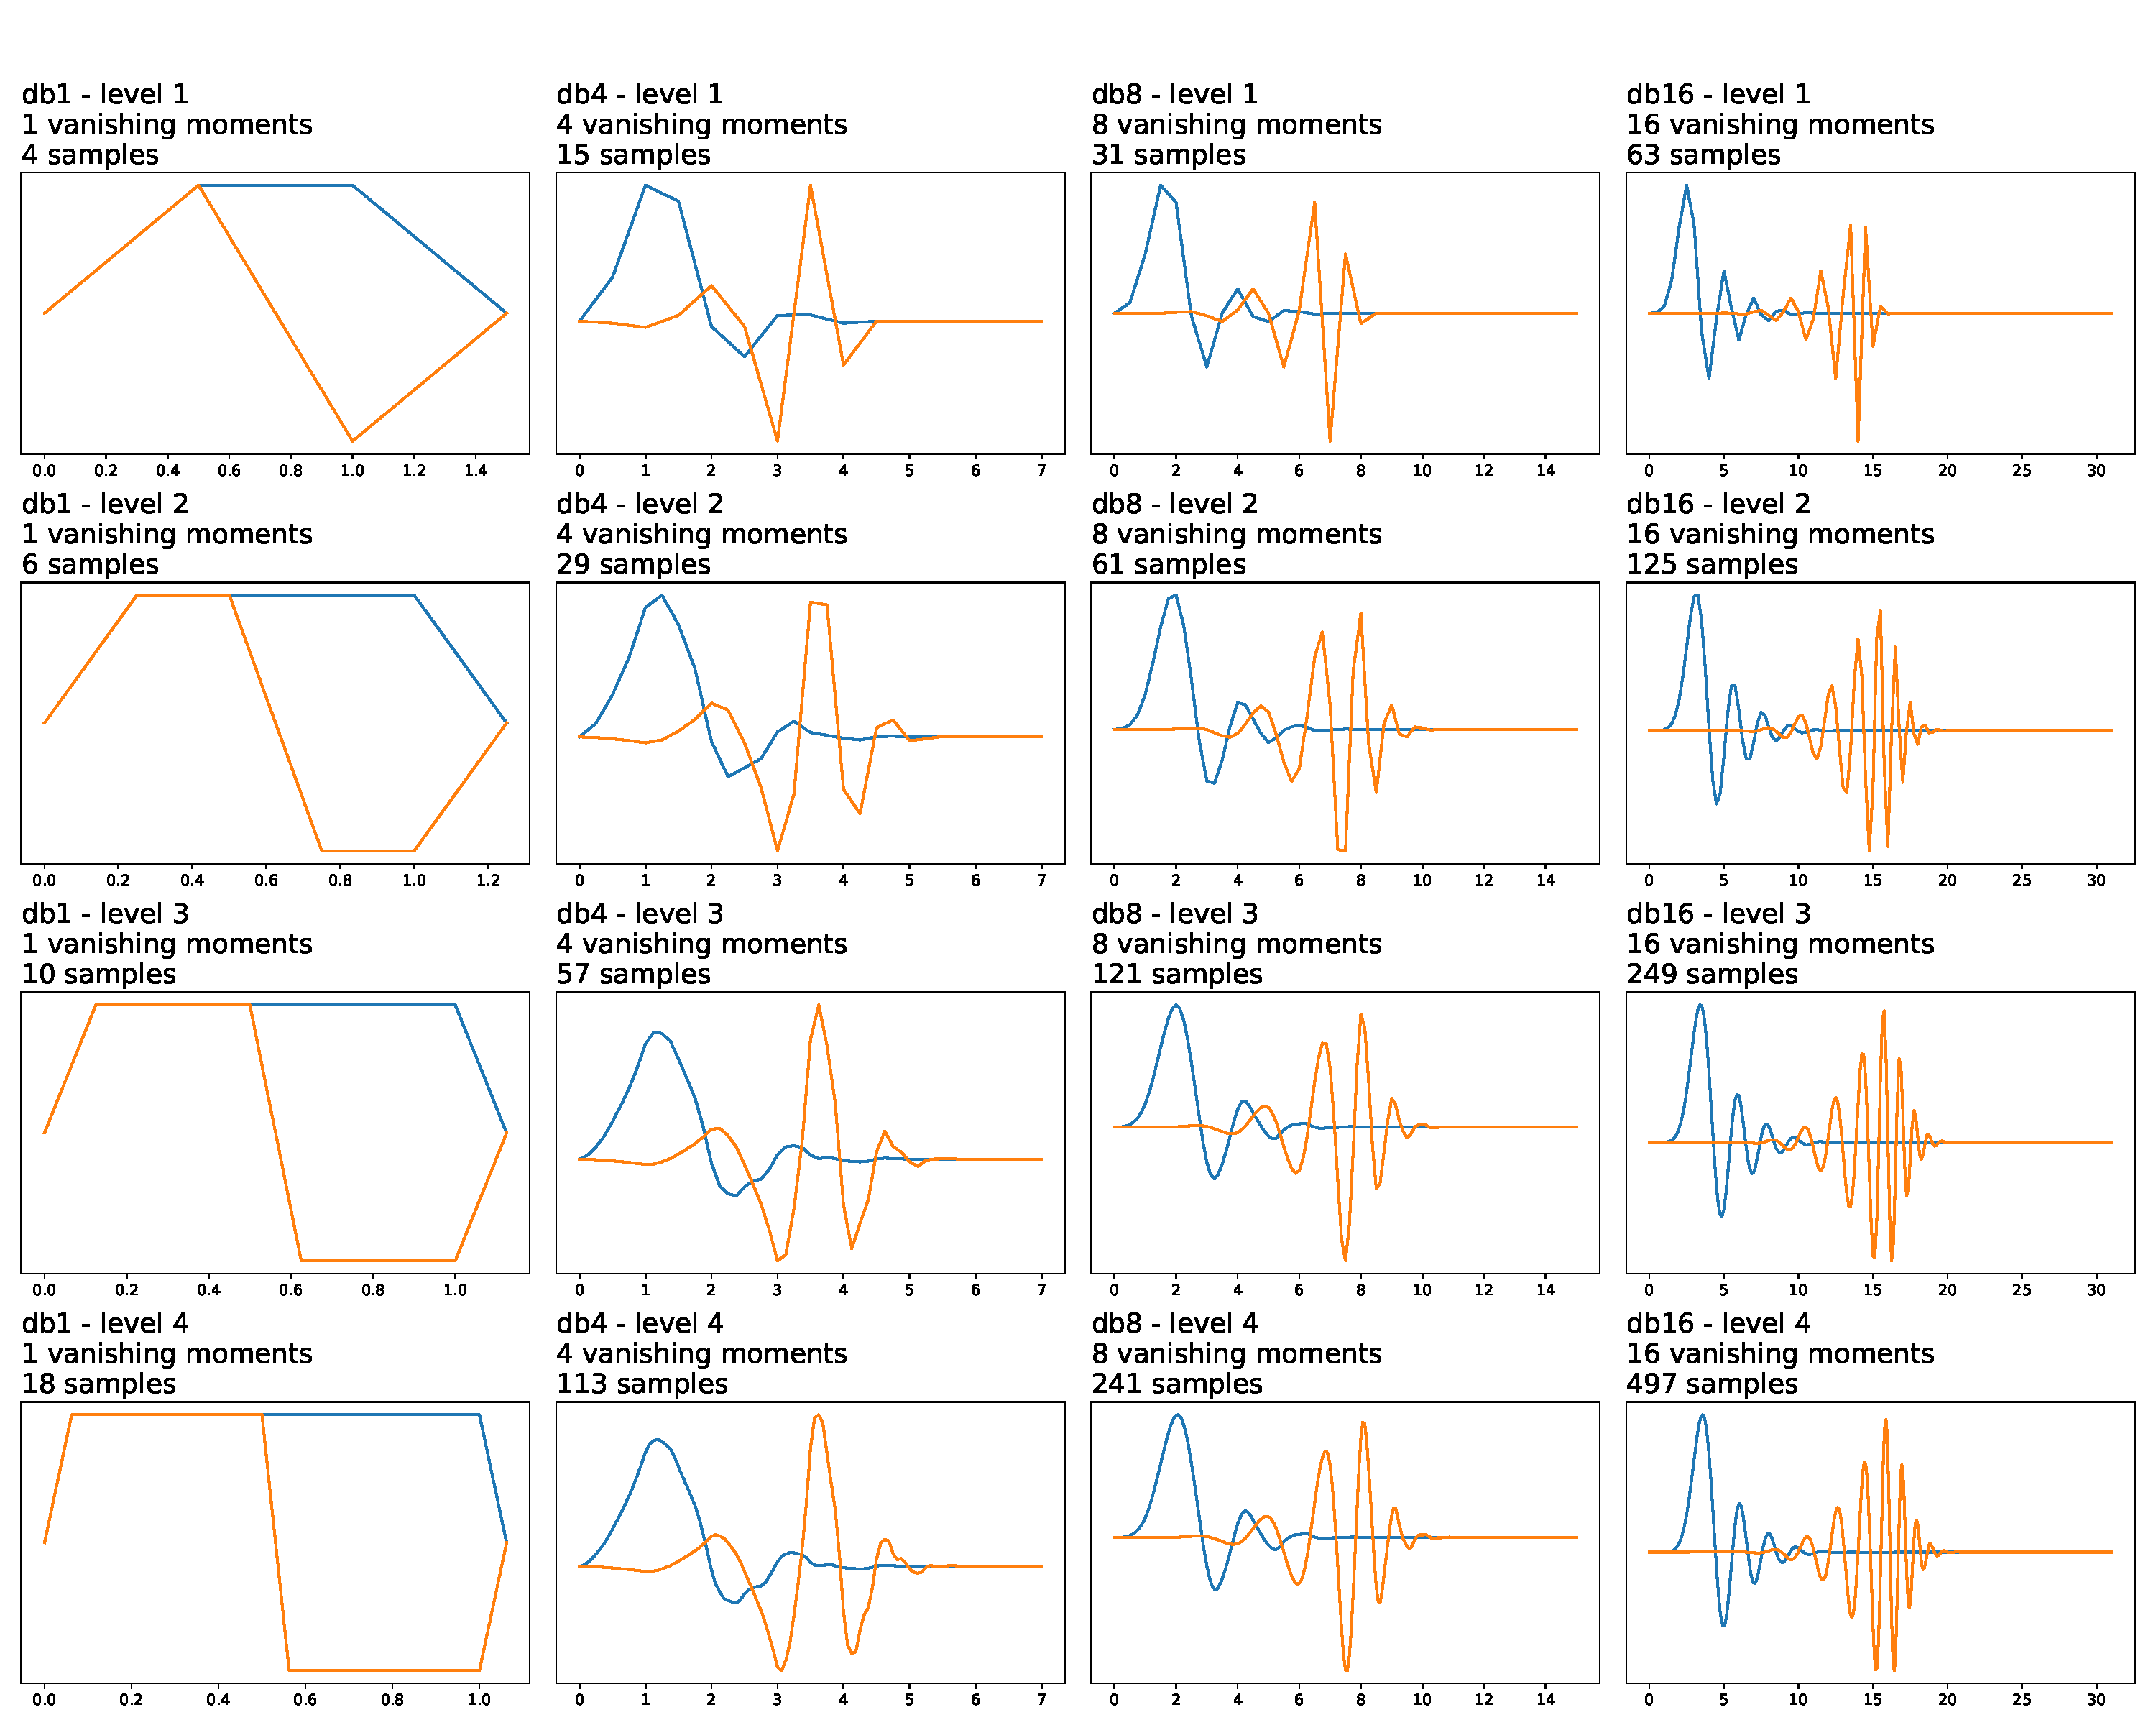
\includegraphics[width=\linewidth]{papers/autotune/sections/frequenzanalyse/images/DauberchiesFamilie.pdf}
	\caption{Eine kleine Auswahl aus der Dauberchies Familie}
	\label{tab:Dauberchies}
\end{table}

Das Ergebnis der Diskreten Wavelet-Tranformation ist in der Grafik \ref{fig:sin-sweep} wiedergegeben. Man sieht eine klare verschlechterung der Ergebnisse im vergleich mit der cwt Analyse aus \ref{fig:STFTCWT} im Frequenzbereich. Man erkennt nur die jeweiligen Oktaven die in der Zeit dargestellt werden. Für eine genauere Analyse sind diese ergebnisse jedoch unbrauchbar.  

\begin{figure}[!ht]
	\centering
	\includegraphics[width=\linewidth]{papers/autotune/sections/frequenzanalyse/images/sweepdwt.jpg}
	\captionof{figure}{Diskrete Wavelet Analyse des Sinus Sweep 0-400$Hz$}\label{fig:sin-sweep}
\end{figure}%


\newpage


\newpage

\section{Frames zur Analyse}
\rhead{Frames zur Analyse}
%
% frames.tex
%
% (c) 2019 Prof Dr Andreas Müller, Hochschule Rapperswil
%
\section{Frames
\label{section:frames}}
\rhead{Frames}
Eine orthonormierte Basis eines Hilbertraumes ist sehr starr.
Es ist nicht möglich, auch nur einen einzigen Vektor ein kleines
Bisschen zu ändern, ohne die Eigenschaften, die zum Satz~\ref{satz:parseval}
geführt haben, zu zerstören.
Im Hinblick auf die numerische Behandlung von Signalen ist das
ein unerwünschter Zustand.
Rundungsfehler werden unvermeidlich dazu führen, dass solche strengen
Strukturen nur näherungsweise im Computer nachgebildet werden 
können.

Die Zerlegung eines Vektors $v$ in einer Orthonormalbasis enthält keine
Redundanz.
Geht einer der Koeffizienten $\hat{v}_k$ verloren, gibt es keine
Chance, den Vektor zu rekonstruieren.
Auch diese Situation ist unerwünscht, denn durch Rundungsfehler geht
mindestens ein Teil der Information in einem Koeffizienten verloren.
Wir suchen daher nach einer Verallgemeinerung des Basis-Begriffs, welche
auf kontrollierte Weise Redundanz in die Koeffizienten $\hat{v}_k$
bringt und damit eine robustere Konstruktion ermöglicht.

\subsection{Ein geometrisches Beispiel
\label{subsection:hexagon}}
\begin{figure}
\centering
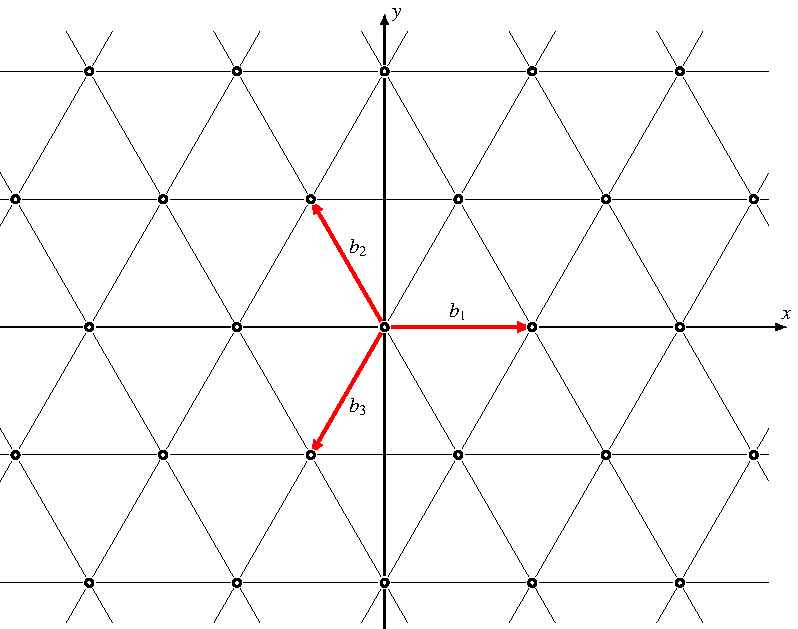
\includegraphics{chapters/1-geometrie/images/hexagon.pdf}
\caption{Sechseck-Gitter in der Ebene zum Frame $\{b_1,b_2,b_3\}$.
\label{geometrie:hexagon:image}}
\end{figure}
Wir suchen ein geeignetes Koordinatensystem, um ein Problem über
Bienenwaben in der Ebene zu lösen.
Dazu gehört das hexagonale Gitter in Abbildung~\ref{geometrie:hexagon:image}.
Selbstverständlich kann dafür das übliche rechtwinklige Koordinatensystem
verwendet werden, aber die Ecken eines Sechsecks shaben darin die nicht
sehr symmetrischen Koordinaten
\begin{center}
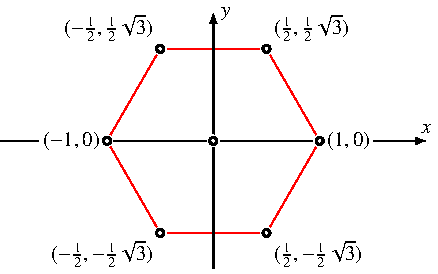
\includegraphics{chapters/1-geometrie/images/hexagon1.pdf}
\end{center}
(Siehe auch Abbildung~\ref{geometrie:hexagon:image}).
Eine bessere Variante ist das Koordinatensystem auf der Basis der beiden
Basisvektoren (in kartesischen Koordinaten)
\[
b_1 = \begin{pmatrix} 1\\0\end{pmatrix}
\qquad
\text{und}
\qquad
b_2 = \begin{pmatrix} -\frac12\\\frac12\sqrt{3}\end{pmatrix}.
\]
In diesem Koordinatensystem haben die Ecken des Sechsecks die Koordinaten
\begin{center}
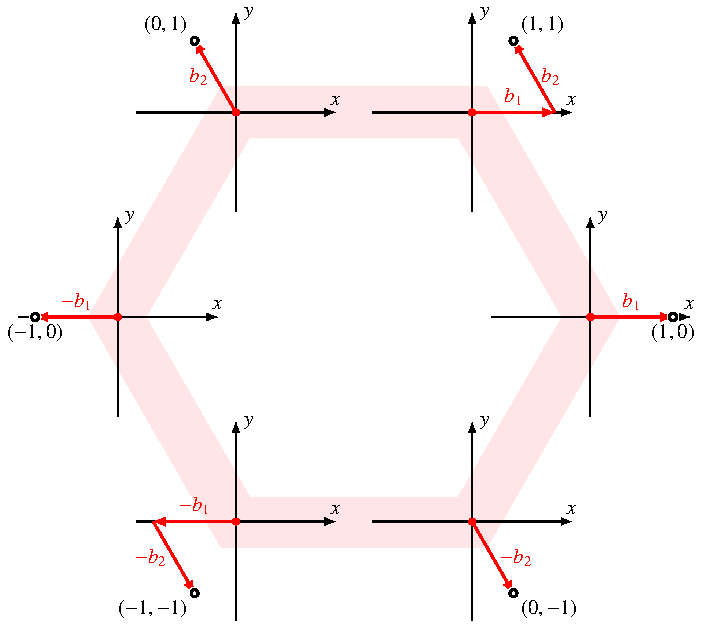
\includegraphics{chapters/1-geometrie/images/hexagon2.pdf}
\end{center}
%\begin{center}
%\begin{tikzpicture}
%\def\a{1.8}
%\foreach \p in {0,60,...,360}{
%	\draw[line width=0.1pt] ({\a*cos(\p)},{\a*sin(\p)})--
%		({\a*cos(\p+60)},{\a*sin(\p+60)});
%}
%\foreach \p in {0,60,...,300}{
%	\fill[color=white] ({\a*cos(\p)-0.65},{\a*sin(\p)-0.25})
%		rectangle ({\a*cos(\p)+0.65},{\a*sin(\p)+0.25});
%}
%
%\node at (0,0) {$0$};
%\node at ({\a},0) {$(1,0)$};
%\node at ({-\a},0) {$(-1,0)$};
%\node at ({0.5*\a},{\a*sqrt(3)/2}) {$(1,1)$};
%\node at ({0.5*\a},{-\a*sqrt(3)/2}) {$(0,-1)$};
%\node at ({-0.5*\a},{\a*sqrt(3)/2}) {$(0,1)$};
%\node at ({-0.5*\a},{-\a*sqrt(3)/2}) {$(-1,-1)$};
%\end{tikzpicture}
%\end{center}
%\begin{align*}
%&      &&(0,1)  &&(1,1)&&     \\
%&(-1,0)&&       &&      &&(1,0)\\
%&      &&(-1,-1)&&(0,-1)&&
%\end{align*}
Was bereits viel besser aussieht.
Trotzdem ist auch dies noch nicht ganz zufriedenstellend. 
Zum Beispiel sind die Ecken links oben und rechts unten direkt durch den
Basisvektor $b_2$ darstellbar, die Ecken rechts oben und links unten
dagegen nur durch eine Linearkombination.
Wir könnten natürlich auch die linke untere Ecke als Basisvektor nehmen,
dann würde einfach die linke obere Ecke speziell.
In dieser Situation lässt es sich also mit einer Basis gar nicht erreichen,
dass alle Eckpunkte sich auf einfache Art darstellen lassen.

Verzichten wir jedoch daruf, dass die Vektoren linear unabhängig sein müssen,
können wir also ``Basis'' die drei Vektoren (in kartesischen Koordinaten)
\begin{align*}
b_1
&=
\begin{pmatrix}1\\0\end{pmatrix}
&
b_2
&=
\begin{pmatrix}-\frac12\\\frac12\sqrt{3}\end{pmatrix}
&
b_3
&=
\begin{pmatrix}-\frac12\\-\frac12\sqrt{3}\end{pmatrix}
\end{align*}
verwenden.
Die drei Vektoren haben alle die Länge $1$, aber sie sind nicht
orthogonal, sondern haben das Skalarprodukt
\[
\langle b_j,b_k\rangle
=
\begin{cases}
-\frac12&\qquad j\ne k\\
0&\qquad j=k.
\end{cases}
\]
Zu jedem Vektor $v\in\mathbb R^2$ können wir wieder die Koeffizienten
$\hat{v}_k=\langle v,b_k\rangle$ berechnen und damit die Linearkombination
\[
v' = \sum_{k=1}^3 \hat{v}_k\,b_k
\]
bilden,
doch es ist $v\ne v'$.
Wir berechnen die Synthese für die Basisvektoren:
\begin{align*}
b_1'
&=
b_1 - \frac12 b_2 - \frac 12 b_3
=
\frac32b_1
\\
b_2'
&=
-\frac12 b_1 + b_2 -\frac12 b_3
=
\frac32b_2
\\
b_3'
&=
-\frac12b_1-\frac12 b_2 + b_3
=
\frac32b_3
\end{align*}
Die Synthese liefert also nicht den ursprünglichen Vektor, sondern
\begin{equation}
\sum_{k=1}^3 \hat{v}_k b_k = \frac32\,v
\label{geometrie:32beispiel}
\end{equation}
zurück, das $\frac32$-fache davon.
Dies ist bereits ein Ausdruck der Tatsache, dass die Information in den
Koeffizienten $\hat{v}_k$ redundant ist.

Diese Vektoren sind natürlich nicht mehr linear unabhängig, Vektoren
der Ebene können also auf verschieden Art linear aus den $b_k$ kombiniert
werden.
Da $b_1+b_2+b_3=0$ ist, kann man zu den Koeffizienten $\hat{v}_k$
eine beliebige Zahl $\alpha$ hinzuaddieren, und erhält
\[
\sum_{k=1}^3 (\hat{v}_k+\alpha)\, b_k
=
\sum_{k=1}^3 \hat{v}_k\,b_k
+\alpha
\sum_{k=1}^3 b_k
=
\sum_{k=1}^3 \hat{v}_k\,b_k
=
\frac32 v.
\]
Die modifizierten Koeffizienten ergeben also das gleichen synthetisierten
Vektor $\frac32 v$.

Für die Norm des synthetisierten Vektors gilt natürlich
\[
\|v'\|^2
=
\frac94\|v\|^2
=
\sum_{k=1}^3 \hat{v}_k^2 
-
\frac12\sum_{k\ne l} \hat{v}_k\hat{v}_l.
\]
Die modifizierten Koeffizienten ergeben natürlich dieselbe Norm, also
\begin{align*}
\|v'\|^2
&=
\sum_{k=1}^3 (\hat{v}_k+\alpha)^2 
-
\frac12\sum_{k\ne l} (\hat{v}_k+\alpha)(\hat{v}_l+\alpha).
\\
&=
\sum_{k=1}^3 \hat{v}_k^2
+2\alpha \sum_{k=1}^3 \hat{v}_k
+3\alpha^2
-
\frac12\sum_{k\ne l} \hat{v}_k\hat{v}_l
-
\sum_{k\ne l} \hat{v}_k \alpha
-
3\alpha^2
\end{align*}


Was zeichnet die Koeffizienten $\hat{v}_k$ gegenüber den modifizierten
Koeffiziente $\hat{v}_k$ aus?
Im Falle einer Orthonormalbasis konnte man dank der Plancherel-Formel
die Norm eines Vektors mit Hilfe der Quadratsumme der Koeffizienten
berechnen.
Wir berechnen daher
\[
f(\alpha)
=
\sum_{k=1}^n (\hat{v}_k+\alpha)^2
=
\sum_{k=1}^n \hat{v}_k^2 + 2\alpha \sum_{k=1}^3 \hat{v}_k + 3\alpha^2
\]

\subsection{Definition eines Frames}
Nach dem motivierenden Beispiel im vorangegangenen Abschnitt sind wir nun
bereit, eine allgemeine Definition aufzubauen.
Wir wollen also weiterhin die Vektoren eines Vektorraums $V$ mit Hilfe
einer Menge von Vektoren $\{e_k\,|\,1\le k\le n\}$ linear kombinieren,
verlangen aber nicht mehr, dass die Vektoren $e_k$ linear unabhängig sind.
Dies bedeutet natürlich, dass die Darstellung eines Vektors $v\in V$
nicht mehr eindeutig sein wird.

Nicht jede Menge von Vektoren $\{e_k\,|\,1\le k\le n\}$ ist geeignet.
Es muss ja immer noch jeder Vektor dargestellt werden können, das
Erzeugnis der Vektoren muss also der ganze Vektorraum sein:
\[
U
:=
\langle e_k\,|\,1\le k\le n\rangle
=
V.
\]
Wäre das Erzeugnis nur ein echter Unterraum $U\subset V$, dann gäbe es
einen Vektor $b\in V$, der senkrecht steht auf allen $b\perp V$.
Wir fordern daher, dass es keinen Vektor gibt, der auf allen Vektoren $e_k$
senkrecht steht.

Damit die Berechnung effizient bleibt, möchten wir weiterhin nur mit den
Koeffizienten $\hat{v}_k = \langle v,e_k\rangle$ arbeiten müssen.
Für eine Orthonormalbasis hat die Plancherel-Formel gezeigt, dass
\[
\sum_{k=1}^n |\hat{v}_k|^2 = \| v \|.
\]
In der aktuellen Situation können wir nicht mehr erwarten, dass dies 
weiterhin funktioniert.
Wir müssen aber mindestens verlangen, dass die Transformation
\[
\mathcal{T}
\colon
V\to \mathbb R^n
:
v\mapsto \hat{v}_k
\]
stetig ist, dass sich also kleine Änderungen von $v$ ebenfalls
kleinen Änderungen des Vektors der $\hat{v}_k$ auswirken.
Es muss also eine Konstante $B$ geben, so dass
\[
\sum_{k=1}^n |\hat{v}_k|^2
=
\sum_{k=1}^n |\langle v,e_k\rangle|^2
\ge
A \| v \|^2.
\]

Wir müssen aber auch sicherstellen, dass die Rekonstruktion des Vektors $v$
auf stetige Art von den Koeffizienten $\hat{v}_k$ abhängt. 
Eine kleine Änderung der Koeffizienten darf sich nur in beschränkten Änderungen
im rekonstruierten Vektor $v$ auswirken.
Es muss also eine Konstante $B$ geben, so dass
\[
\sum_{k=1}^n |\hat{v}_k|^2
=
\sum_{k=1}^n |\langle v,e_k\rangle|^2
\le
B \| v \|^2
\]
gilt.

Damit haben wir alle Elemente zusammen für die folgende Definition,
die auch für unendlichdimensionale Hilberträume funktioniert.

\begin{definition}
\label{definition:frame}
Eine Teilmenge $\{ e_k\,|\, k\in K\}\subset V$ heisst ein {\em Frame},
wenn es zwei von $0$ verschiedene Konstanten $A$ und $B$ gibt, so dass
\[
A\|v\|^2 \le \sum_{k\in K} |\langle v, e_k\rangle|^2 \le B \| v\|^2
\]
gilt für jeden Vektor $v\in V$.
Die Konstanten $A$ und $B$ heissen die {\em Framekonstanten} des Frames.
Das Frame heisst {\em straff}, wenn $A=B$ ist.
\end{definition}

\begin{beispiel}
Das Beispiel von Abschnitt~\ref{subsection:hexagon} ist ein Frame.
Die Formel \eqref{geometrie:32beispiel} zeigt, dass die Framekonstanten
des Frames $A=B=\frac32$ ist.
Das Frame ist also sogar straff.
\end{beispiel}

In der Definition wird nicht erwähnt, dass die Vektoren des Frames den
ganzen Raum aufspannen müssen.
Diese Eigenschaft folgt jedoch direkt aus der Definition eines Frames,
wie der folgende Satz zeigt.

\begin{satz}
Ist $\mathcal{B}=\{ e_k\,|\, k\in K\}$ ein Frame des Hilbertraumes $V$
mit Framekonstanten $A$ und $B$, dann gibt es keinen Vektor $v\in V$,
der auf allen Vektoren $e_k$ senkrecht steht.
\end{satz}

\begin{proof}[Beweis]
Nehmen wir an, es gäbe einen Vektor $v\in V$ mit $\langle v,e_k\rangle=0$
für alle $k\in K$.
Dann folgt aus den Frame-Ungleichungen
\[
\| v \|^2 \le \frac1{A} \sum_{k\in K} |\langle v,e_k\rangle|^2 = 0
\qquad\Rightarrow\qquad
v=0.
\]
Der Nullvektor ist also der einzige Vektor, der auf allen Framevektoren
senkrecht steht.
\end{proof}

Eine orthonormierte Basis war die bevorzugte Wahl für eine Basis, weil
sich damit die Transformation $\mathcal{T}$ besonders leicht invertieren
lässt.
Der Satz~\ref{satz:parseval} hat gezeigt, dass die Transformation %$\mathcal{T}$
eine Isometrie ist, insbesondere gilt
\[
\|v\|^2
=
\sum_{k\in K} |\hat{v}_k|^2
=
\sum_{k\in K} |\langle v,e_k\rangle|^2.
\]
Dies bedeutet, dass eine orthonormierte Basis ein straffes Frame mit
Framekonstanten $A=B=1$ ist.
Umgekehrt drängt sich die Frage auf, ob straffe Frames oder spezielle
Werte der Frame-Konstanten eine besondere Bedeutung für die Invertierbarkeit
haben.

\begin{figure}
\centering
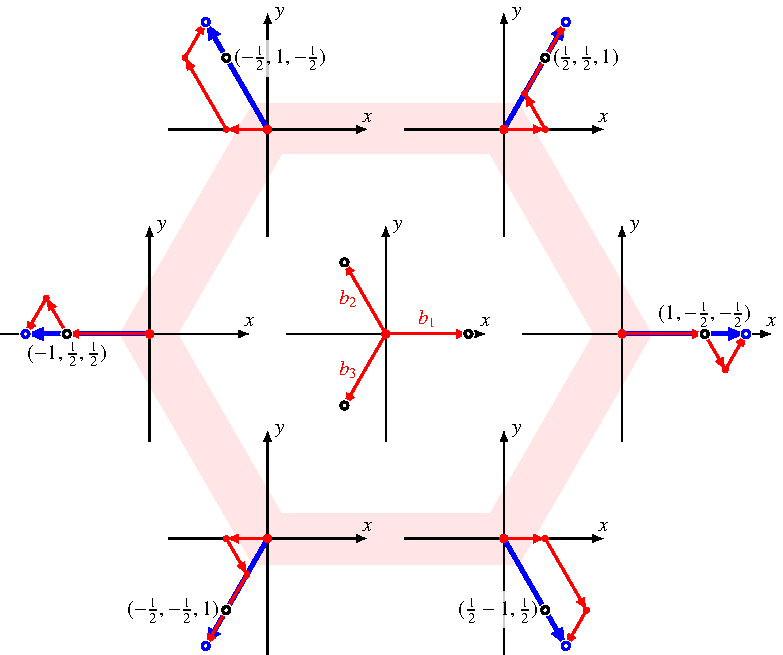
\includegraphics{chapters/1-geometrie/images/hexagon3.pdf}
\caption{Rekonstruktion bei einem straffen Frame.
Das Frame bestehend aus den Vektoren $\{b_1,b_2,b_3\}$ ist straff
mit der Framekonstanten $A=\frac32$.
Die mit den Skalarprodukten gewichtete Linearkombination der
Framevektoren liefert nicht den ursprünglichen Vektor zurück, sondern
einen Vektor, der mit der Framekonstanten multipliziert wird.
Gezeigt wird dies für die sechs Ecken des Hexagons.
Die Skalarprodukte mit den Framevektoren, die Framekoordinaten, sind
als Zahlentripel bei jedem Punkt angegeben.
Die roten Vektorpfade stellen die Linearkombination dar, die blauen
Vektoren die Summe.
\label{geometrie:hexagon:rekonstruktion}}
\end{figure}

\subsection{Allgemeine Frames}
Die Wahl der Indexmenge $K$ in der Definition~\ref{definition:frame}
war einigermassen willkürlich.
Schon bei der Fouriertransformation ist eine solche diskrete Menge
für die Indizierung der Vergleichsfunktionen nicht mehr ausreichend.
Dort werden nämlich die Funktion $e^{i\omega t}$ mit $\omega\in\mathbb R$
verwendet.
Auch die geplante Anwendung auf Wavelets ist davon betroffen.
Dort wollen wir mit Funktionen $\psi_{a,b}$ vergleichen, die 
skalierte und verschobene Versionen eines Mutter-Wavelets $\psi$ sind,
mit Skalierungsfaktor $a\in\mathbb R^*$ und $b\in \mathbb R$.

Lässt man eine beliebige Indexmenge zu, ist die Definition der
Transformation $T$
\[
k
\mapsto
(Tv)(k) = \langle v,e_k\rangle
\]
als komplexwertige Funktion auf $K$ immer noch sinnvoll.
Für eine überabzählbare Indexmenge $K$ ist die Summe 
\[
\sum_{k\in K} |\langle v,e_k\rangle|^2,
\]
die in der Definition eines Frames auftritt, schlicht sinnlos.
Wir stehen hier also vor einem ähnlichen Problem wie bei der Frage,
wie man aus dem Raum der Signale auf $\mathbb R$ einen Hilbertraum machen kann.
Diese Frage wird in Kapitel~\ref{chapter:fourier} im Detail beantwortet.

Nehmen wir für den Moment an, dass es gelungen ist, eine Hilbertraum $H$
von Funktionen auf $K$ zu konstruieren.
Die Frame-Ungleichung kann dann mit Hilfe der Norm von $H$ formuliert
werden, sie lautet
\[
A\|v\|^2 \le \|Tv\|^2 \le B\|v\|^2.
\]
Die Norm in der Mitte ist als Norm in $H$ zu lesen.
Diese Ungleichungen sagen immer noch aus, dass kein Vektor $v\in V$ bei
der Transformation $T$ ``unsichtbar'' wird.
Wäre nämlich $Tv=0$ in $H$, dann wäre auch $\|Tv\|=0$ und damit
$\|v\|=0$.
Die Frame-Ungleichung stellt also sicher, dass die Abbildung $T$ 
injektiv und damit potentiell invertierbar ist.

Es ist aber keinesfalls garantiert, dass das Bild der Transformation $T$
den ganzen Hilbertraum $T$ abdeckt, ganz im Gegenteil.
Schon im Beispiel in Abschnitt~\ref{subsection:hexagon} wurde gezeigt,
dass die mit Hilfe eines Frames gefundenen Koeffizienten redundant sind.
Alle Vektoren der Menge
\[
\left\{
\left.
\begin{pmatrix}\hat{v}_1\\\hat{v}_2\\\hat{v}_3\end{pmatrix}
+\alpha\begin{pmatrix}1\\1\\1\end{pmatrix}
\,
\right|\,
\alpha \in\mathbb R
\right\}
\]
beschreiben den gleichen Punkt in der Ebene, aber nur einer davon 
wird von der Transformation $T$ erreicht.
Dies entspricht natürlich genau dem, was man erwartet: der Bildraum
der Ebene $\mathbb R^2$ unter der Abbildung $T$ ist ein zweidimensionaler
Teilraum des $\mathbb R^3$.

Die Abbildung $T$ wird daher im Allgemeinen nicht invertierbar sein, aber
wir dürfen hoffen, dass es eine Formel gibt, mit der man aus $Tv$ den 
Vektor $v$ rekonstruieren kann.
Im Falle des Beispiels war dies die Formel
\[
v = \frac23 \sum_{k=1}^3 \langle v,e_k\rangle \, e_k.
\]
Für ein beliebiges Frame ist so eine Formel natürlich wieder wegen
der Summe nicht sinnvoll.
Dach in Kapitel~\ref{chapter:fourier} werden wir sehen, dass sie sich
oft durch eine Integralformel ersetzen lässt.
Die Konstruktion eines solchen vektorwertigen Integrals ist allerdings
etwas subtil, wird kehren zu dieser Problematik im Kapitel~\ref{chapter:cwt}
zurück.



\newpage

\section{Schlussfolgerung}
\rhead{Schlussfolgerung}

\printbibliography[heading=subbibliography]
\end{refsection}
